\documentclass[11pt,a4paper,titlepage]{article}
\usepackage[utf8]{inputenc}
\usepackage[english,polish]{babel}
\usepackage[T1]{fontenc}
\usepackage{polski}
\usepackage[math,light]{anttor}
\usepackage{amsmath}
\usepackage{amsfonts}
%\usepackage{amssymb}
\usepackage{graphicx}
\usepackage{sidecap}
%\usepackage{wrapfig}
\usepackage{epstopdf}
\usepackage{booktabs}
\usepackage{forloop}
\usepackage[left=3cm,right=3cm,top=3cm,bottom=3cm]{geometry}
\usepackage[framed,numbered,autolinebreaks]{mcode}
\usepackage[colorlinks=false,hidelinks,urlcolor=blue,citecolor=green]{hyperref}
\usepackage{fancyhdr}
\usepackage{lastpage}
\usepackage{array}
\usepackage{hhline}
\usepackage{multirow}
\usepackage {float}
\usepackage{subfig}
\usepackage{enumerate}%[I], numerki, [(a)]
%ustawienie poziomów wypunktowania do wyboru: $\bullet$, $\cdot$, $\diamond$, $-$, $\ast$ and $\circ$ 
\renewcommand{\labelitemi}{$\diamond$}
\renewcommand{\labelitemii}{$\bullet$}
\renewcommand{\labelitemiii}{$-$}
\renewcommand{\labelitemiv}{$\ast$}


\AtBeginDocument{

	\renewcommand{\tablename}{Tabela}

	\renewcommand{\figurename}{Rys.}
}

%tabelki
\usepackage{tabularx}
\newcolumntype{A}{>{\centering\arraybackslash}X}
\newcolumntype{B}{>{\centering\arraybackslash} m{0.4\textwidth} }


% --- < bibliografia > ---
\usepackage[
style=numeric,
sorting=none,
% Zastosuj styl wpisu bibliograficznego właściwy językowi publikacji.
language=auto,
autolang=other,
% Zapisuj datę dostępu do strony WWW w formacie RRRR-MM-DD.
urldate=iso8601,
% Nie dodawaj numerów stron, na których występuje cytowanie.
backref=false,
% Podawaj ISBN.
isbn=true,
% Nie podawaj URL-i, o ile nie jest to konieczne.
url=false,
% Ustawienia związane z polskimi normami dla bibliografii.
maxbibnames=3,
% Jeżeli używamy BibTeXa:
backend=bibtex
]{biblatex}
% --- < bibliografia > --- Koniec

\usepackage{csquotes}
\DeclareQuoteAlias{croatian}{polish} % Ponieważ `csquotes` nie posiada polskiego stylu, można skorzystać z mocno zbliżonego stylu chorwackiego.

\addbibresource{bibliografia.bib}

\pagestyle{fancy}
\fancyhf{}
\fancyhead[R]{\slshape{\small \rightmark}}
\fancyfoot[R]{Wahadło odwrócone}
\fancyhead[L]{P. Merynda, M. Podsiadło, P. Zielonka}     
\fancyfoot[L]{Strona \thepage \hspace{1pt} z\hspace{1pt} \pageref*{LastPage}}    
\renewcommand{\headrulewidth}{1pt}
\renewcommand{\footrulewidth}{1pt}


\begin{document}

\begin{titlepage}

\newcommand{\HRule}{\rule{\linewidth}{0.5mm}} % Defines a new command for the horizontal lines, change thickness here

\center % Center everything on the page
 
%----------------------------------------------------------------------------------------
%	HEADING SECTIONS
%----------------------------------------------------------------------------------------

\textsc{\LARGE Akademia Górniczo - Hutnicza im. Stanisława Staszica}\\[0.5cm]

\includegraphics[scale=0.6]{agh}\\[1cm] % Name of your university/college
\textsc{\Large Wydział Elektrotechniki, Automatyki, Informatyki i Inżynierii Biomedycznej}\\[0.5cm] % Major heading such as course name
\textsc{\large Katedra Automatyki i Inżynierii Biomedycznej}\\[0.5cm]
\textsc{ Kierunek: Automatyka i robotyka}\\[0.5cm] % Minor heading such as course title

%----------------------------------------------------------------------------------------
%	TITLE SECTION
%----------------------------------------------------------------------------------------

\HRule \\[0.4cm]
{ \huge \bfseries Laboratorium Problemowe 2\\[1cm]Wahadło odwrócone}\\[0.4cm] % Title of your document
\HRule \\[2.5cm]
 


%----------------------------------------------------------------------------------------
%	DATE SECTION
%----------------------------------------------------------------------------------------

%{\large \today}\\[1.5cm] % Date, change the \today to a set date if you want to be precise

%----------------------------------------------------------------------------------------
%	LOGO SECTION
%----------------------------------------------------------------------------------------

%
\includegraphics[height=70mm]{agh.jpg}%\\[1cm] % Include a department/university logo - this will require the graphicx package
%----------------------------------------------------------------------------------------
%	AUTHOR SECTION
%----------------------------------------------------------------------------------------

\begin{flushleft}
\Large
\emph{Wykonali:}\\
Piotr Merynda\\
Maciej Podsiadło\\
Piotr Zielonka\\[1cm]

% If you don't want a supervisor, uncomment the two lines below and remove the section above
 \emph{Prowadzący:}\\
mgr inż. Dawid Knapik\\[3cm] % Your name
 
\end{flushleft}
%----------------------------------------------------------------------------------------
\end{titlepage}
\clearpage
\setcounter{page}{2}

\section{Wstęp}
Celem projektu była synteza układu regulacji dla systemu wahadła odwróconego na wózku. Wyszczególniono następujące zadania sterowania: doprowadzenie wahadła do górnego, niestabilnego punku równowagi za pomocą algorytmu \textit{swing-up} oraz stabilizację wahadła w niestabilnym punkcie równowagi.

Stanowisko laboratoryjne składa się z wahadła znajdującego się na wózku napędzanym przez silnik DC, enkoderów inkrementalnych sczytujących położenie kątowe wahadła oraz wału silnika. Silnik DC sterowany jest sygnałem PWM. Układ połączony jest z komputerem klasy PC na którym zainstalowany jest system operacyjny Windows, MATLAB R2015b z toolboxami umożliwiającymi automatyczną generację kodu z bloków Simulinka, a także oprogramowanie umożliwiające uruchomienie wygenerowanego kodu w czasie rzeczywistym.


%\begin{figure}
%\centering
%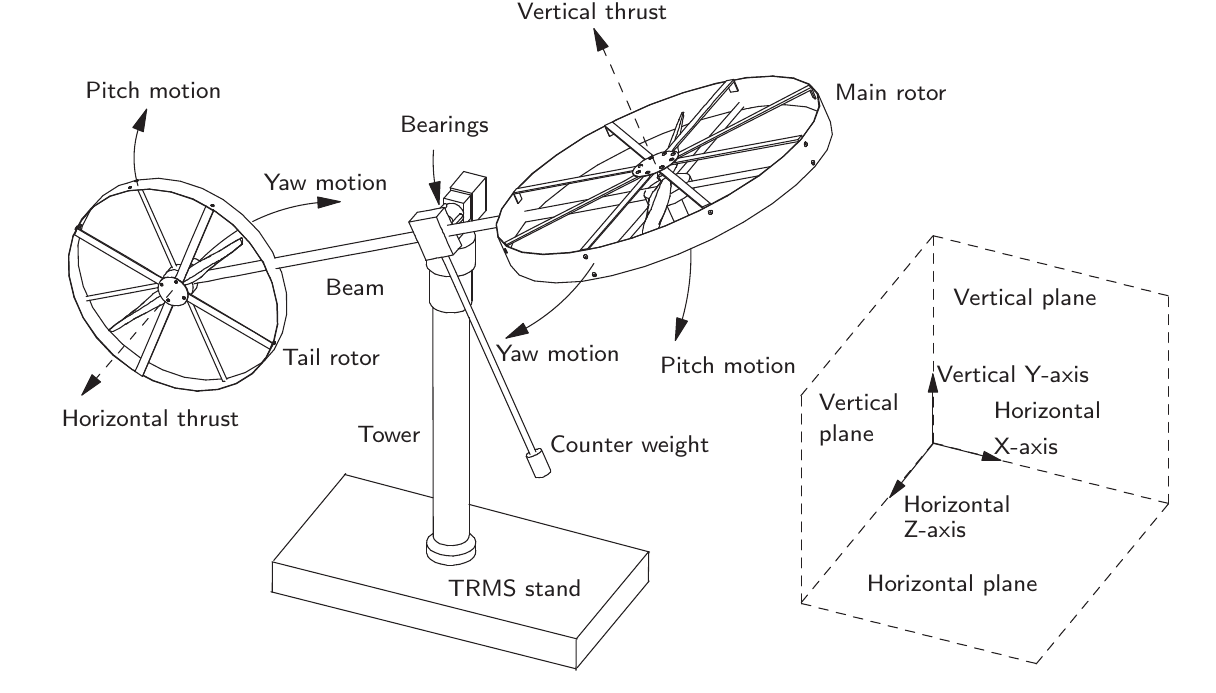
\includegraphics[width=15cm]{obrazy/heli.png}
%\caption{Schemat układu - helikopter na uwięzi}
%\label{fig:heli}
%\end{figure}

\section{Identyfikacja parametrów systemu}
Punktem wyjściowym do rozpoczęcia prac był laboratoryjny model wahadła zbudowany w Simulinku mający następujące sygnały:\\
Wejściowe: sygnał sterujący podawany na silnik (zakres: -0.5 do 0.5), reset enkoderów.\\
Wyjściowe: odczytane z enkoderów położenie kątowe wahadła oraz położenia wózka na szynie, prędkość kątowa wahadła oraz prędkość wózka na szynie (obliczone jako iloraz różnicowy położenia w czasie).\\ 
Przyjęto, że punkt nieciągłości położenia wahadła będzie znajdował się w dolnym, stabilnym położeniu równowagi, natomiast enkodery resetowane będą w lewym (patrząc od strony komputera) skrajnym położeniu wózka na szynie.
\subsection{Obliczenie momentu bezwładności wahadła}
Wahadło składa się z rurki oraz ciężarka znajdującego się na jej końcu. Rozkręcając wahadło zważono oraz zmierzono niezbędne wielkości potrzebne do analitycznego wyliczenia momentu bezwładności wahadła.\\
\noindent\rule[0.2cm]{\textwidth}{1pt}
Masa rurki $m_r=0.02[kg]$\\
Masa ciężarka $m_c=0.011[kg]$\\
Całkowita długość wahadła $d_w=0.495[m]$\\
Odległość od początku rurki do osi obrotu $d_1=0.085[m]$\\
Odległość od osi obrotu do środka masy wahadła $l=0.252[m]$.\\
\noindent\rule[0.5cm]{\textwidth}{1pt}
Rozważając rurkę jako nieskończenie cienki pręt oraz ciężarek jak masę punktową obliczono moment bezwładności wahadła względem osi obrotu: 
\begin{equation}
J_{os} = 2(\frac{m_r}{3}(\frac{d_w-d_1}{d_w}(d_w-d_1)^2+\frac{d_1}{d_w}d_1^2)+m_c(d_w-d_1)^2)
\end{equation}
Na stanowisku wahadło składa się z dwóch identycznych części, stąd współczynnik 2. Po podstawieniu wartości $J_{os} = 0.00557 [kg \cdot m^2]$.\\
Uzyskany wynik postanowiono porównać z wynikiem eksperymentalnym. Unieruchomiwszy wózek nieznacznie wychylono wahadło i zarejestrowano drgania w czasie.  Zmierzono średni okres drgań $T = 1.207s$. Traktując obiekt jako wahadło fizyczne wyliczono moment bezwładności $J_{eksp}$ według znanej zależności:
\begin{equation}
T = 2\pi\sqrt{\dfrac{J_{eksp}}{2(m_c+m_r)gl}}
\end{equation}
gdzie g oznacza przyspieszenie ziemskie.
Otrzymano wynik $J_{eksp} = 0.00565 [kg \cdot m^2]$ zadowalająco bliski analitycznemu.

Aby uprościć model matematyczny systemu policzono moment bezwładności $J_{sm}$ wahadła względem jego środka masy. Wykorzystano twierdzenie Steinera:
\begin{equation}
J_{os} = J_{sm} + 2\cdot(m_c+m_r)\cdot l^2
\end{equation}
Skąd ostatecznie $J_{sm} = 0.00167[kg \cdot m^2]$.
\subsection{Identyfikacja modelu dynamiki wózka}
Przyjmując uproszczony model silnika DC zapisano następujący układ równań:
\begin{align}
u &= Ri + k_e\omega \\
J_{DC}\dot{\omega} &= k_mi - \mu\omega
\end{align}
gdzie:\\
u - napięcie podane na silnik,\\
R - rezystancja wirnika,\\
i - natężenie prądu,\\
$\omega$ - prędkość kątowa wirnika,\\
$k_e$ - stała elektryczna silnika,\\
$k_m$ - stała mechaniczna silnika,\\
$J_{DC}$ - moment bezwładności układu względem osi obrotu silnika.\\
$\mu$ - wypadkowy współczynnik tarcia układu\\
Eliminując \textit{i}:
\begin{equation}
\label{eq:dynW}
\dot{\omega}=-\frac{k_ek_m+\mu R}{J_{DC}R}\omega+\frac{k_m}{J_{DC}R}u
\end{equation}
Aby uniknąć konieczności wyznaczania wszystkich wielkości występujących w równaniu \ref{eq:dynW} postanowiono zidentyfikować dwie stałe $c_1$ oraz $c_2$. Mając na uwadze, że prędkość wózka na szynie $\dot{z}$ jest proporcjonalna do prędkości obrotowej wirnika:
\begin{equation}
\label{eq:zz}
\ddot{z}=-c_1\dot{z}+c_2u
\end{equation}
Minimalizując całkę z kwadratu różnicy pomiędzy rzeczywistym przebiegiem a modelem opartym o wyżej wymienione stałe otrzymano rezultat:
\begin{figure}[H]
\centering
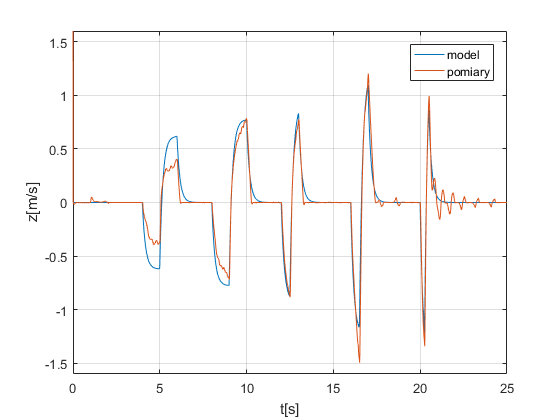
\includegraphics[width=12cm]{obrazy/pr_woz.png}
\caption{Porównanie modelu dynamiki wózka z pomiarami}
\label{fig:wozek}
\end{figure}
dla $c_1 = 5.8$, $c_2 = -18$. 

Pominięto wpływ wahadła na ruch wózka. Uproszczenie to jest szczególnie uzasadnione w momencie kiedy wahadło znajdować się będzie w niestabilnym punkcie równowagi. Na rysunku \ref{fig:wozek} widać, że przy mniejszych prędkościach występują większe rozbieżności pomiędzy modelem a pomiarami, co spowodowane jest bardziej znaczącym wpływem tarcia statycznego, którego nie uwzględniono do tej pory w modelu.

\section{Model matematyczny}
Przyjmując zerowy kąt wychylenia $\phi$ w górnym położeniu równowagi wahadła założono, że wartości rosną w kierunku matematycznie ujemnym (zgodnie z ruchem wskazówek zegara).  
\begin{figure}[H]
\centering
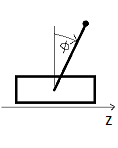
\includegraphics[width=3cm]{obrazy/wozek2.png}
\caption{Schemat wahadła na wózku}
\label{fig:www}
\end{figure}
Na rysunku \ref{fig:www} zaznaczono kierunki mierzenia kąta wychylenia wahadła oraz położenia wózka.
\subsection{Wyprowadzenie modelu}
Rozważając wahadło oddzielnie od wózka wprowadzono siły reakcji więzów $H(t)$ oraz $V(t)$. Pierwsza z nich działa w kierunku poziomym wzdłuż szyny, natomiast druga prostopadle do niej.
\begin{equation}
\label{eq:fiz}
\begin{aligned}
&m\dfrac{d^2}{dt^2}[z(t)+l\sin \phi(t)] = H(t)\\
&m\dfrac{d^2}{dt^2}[l\cos \phi(t)] = V(t)-mg\\
&J_{sm}\dfrac{d^2\phi(t)}{dt^2} = lV(t)\sin \phi(t)-lH(t)\cos \phi(t)
\end{aligned}
\end{equation}
Równania \ref{eq:fiz} są wynikiem zastosowania drugiej zasady dynamiki Newtona dla kolejno: sił działających na wahadło w poziomie, sił pionowych oraz momentów obrotowych względem środka ciężkości wahadła. Symbol $m$ oznacza całkowitą masę wahadła.

Po przekształceniach układu \ref{eq:fiz}, mając na uwadze równanie dynamiki wózka \ref{eq:zz} otrzymano równanie:
\begin{equation}
\label{eq:rowNonLin}
\ddot{\phi}=\dfrac{mgl}{J_{sm}+ml^2}\sin\phi+\dfrac{mlc_1}{J_{sm}+ml^2}\dot{z}\cos\phi-\dfrac{mlc_2}{J_{sm}+ml^2}u\cos\phi
\end{equation}
W celu sprawdzenia poprawności wyprowadzonego modelu wygenerowano przykładowe sterowanie oraz porównano zarejestrowane przebiegi z modelowymi:
\begin{figure}[H]
\centering
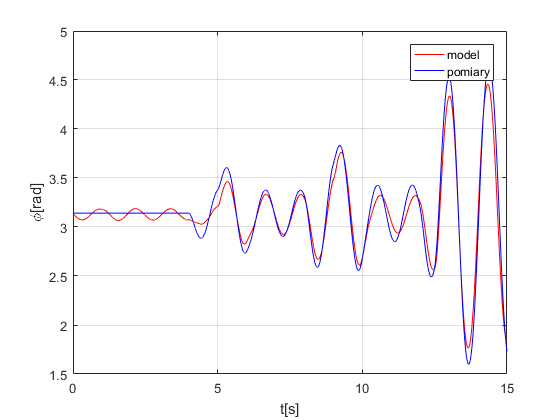
\includegraphics[width=12cm]{obrazy/rad.png}
\caption{Położenie kątowe wahadła}
\label{fig:poW}
\end{figure}
\begin{figure}[H]
\centering
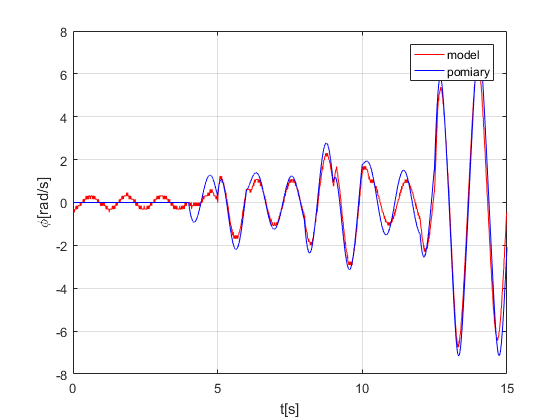
\includegraphics[width=12cm]{obrazy/radPerSec.png}
\caption{Prędkość kątowa wahadła}
\label{fig:prW}
\end{figure}
\subsection{Równania stanu}
Zidentyfikowany model dynamiki wózka oraz dynamiki wahadła pozwala na zapis równań stanu systemu w standardowej formie $\dot{\textbf{x}}=f(\textbf{x},u)$. Przyjmując następujące zmienne stanu:
\begin{equation}
\label{eq:rStan1}
\begin{aligned}
x_{1} = \phi \\
x_{2} = \dot{\phi} \\
x_{3} = z\\
x_{4} = \dot{z}
\end{aligned}
\end{equation}
nieliniowe równania stanu przyjmują postać:
\begin{equation}
\label{eq:rStan2}
\begin{aligned}
&\dot{x_{1}} = x_2 \\
&\dot{x_{2}} = \dfrac{mgl}{J_{sm}+ml^2}\sin x_1+\dfrac{mlc_1}{J_{sm}+ml^2}x_4\cos x_1-\dfrac{mlc_2}{J_{sm}+ml^2}u\cos x_1 \\
&\dot{x_{3}} = x_4\\
&\dot{x_{4}} = -c_1x_4+c_2u
\end{aligned}
\end{equation}

%\input{modelMat}
%\input{regulacjaPID}
\section{Regulator LQR}
\subsection{Linearyzacja}
W kolejnym etapie badań podjęto się implementacji regulatora liniowo-kwadratowego. LQR jest regulatorem optymalnym (minimalizuje funkcję kosztu dla systemu zlinearyzowanego) co niezwykle zwiększa jego rangę i wartość w zastosowaniach. Jak sama nazwa wskazuje LQR stosowany jest do systemu opisanego przez liniowe równania różniczkowe (w naszym przypadku równania zlinearyzowane wokół niestabilnego punktu równowagi), a minimalizowana funkcja kosztu ma postać kwadratową. Postawiony problem można zapisać w sposób następujący:
\begin{equation}
\begin{aligned}
&0 = f(x_{0},u_{0}) \\    
&x_{0} = [0, 0, 0, 0]^T \\
&u_{0} = 0
\end{aligned}
\end{equation}
System zlinearyzowany w otoczeniu przedstawionego punktu równowagi:
\begin{equation}
\dot{x} = A\left( x-x_{0}\right)  + B\left( u-u_{0}\right)     
\end{equation}
gdzie
\begin{equation}
\label{eq:nabla}
\begin{aligned}
A = \bigtriangledown_{x}f(x_{0},u_{0})  \\
B = \bigtriangledown_{u}f(x_{0},u_{0})
\end{aligned}
\end{equation}
Różniczkując równania stanu \ref{eq:rStan} zgodnie z \ref{eq:nabla}:
\begin{equation}
\label{eq:AB}
\begin{aligned}
&\mathbf{A} =
\left( \begin{array}{cccc}
0 & 1 & 0 & 0 \\
\dfrac{mgl}{J_{sm}+ml^2} & 0 & 0 & \dfrac{mlc_1}{J_{sm}+ml^2} \\
0 & 0 & 0 & 1 \\
0 & 0 & 0 & -c_1
\end{array} \right)
&\mathbf{B} =
\left( \begin{array}{cccc}
0 \\
-\dfrac{mlc_2}{J_{sm}+ml^2} \\
0 \\
c_2
\end{array} \right)
\end{aligned}
\end{equation}
a następnie podstawiając wartości do równania \ref{eq:AB} otrzymano:
\begin{equation}
\label{eq:ABwar}
\begin{aligned}
&\mathbf{A} =
\left( \begin{array}{cccc}
0 & 1 & 0 & 0 \\
27.31 & 0 & 0 & 16.15 \\
0 & 0 & 0 & 1 \\
0 & 0 & 0 & -5.8
\end{array} \right)
&\mathbf{B} =
\left( \begin{array}{cccc}
0 \\
50.11 \\
0 \\
-18
\end{array} \right)
\end{aligned}
\end{equation}
Funkcja kosztu jest postaci:
\begin{equation}
Q(u) = \int\limits_{0}^{\infty}  \left( x-x_{0}\right)^TW\left( x-x_{0}\right) + R\left( u-u_{0}\right)^2  dt
\label{eq:cost}  
\end{equation}
Zdecydowano się rozwiązywać problem LQ z nieskończonym horyzontem czasowym, aby uniknąć obliczania online różniczkowego równania Riccatiego. Dzięki takiemu podejściu wyliczenie wzmocnienia regulatora sprowadza się do rozwiązania algebraicznego równania Riccatiego. Pakiet MATLAB oferuje funkcję \textit{lqr(A,B,W,R)}, która rozwiązuje ten problem zwracając gotową macierz K. Półdodatnio określoną macierz W oraz dodatnio określoną macierz (w przypadku układu SIMO - skalar) R dobierano eksperymentalnie w taki sposób, aby regulator jak najszybciej kompensował odchyłki od położenia równowagi przy jednoczesnym uwzględnieniu ograniczeń narzuconych na sterowanie. Sterowanie podawane na obiekt jest postaci:
\begin{eqnarray}
\label{eq:u}
u(t) = -Kx(t)\\
u\in[-0.5, 0.5]    
\end{eqnarray}
Przetestowano różne konfiguracje macierzy W oraz R. Subiektywnie stwierdzono, że system zachowuje się najlepiej dla wartości:
\begin{equation}
\begin{aligned}
&\mathbf{W} =
\left( \begin{array}{cccc}
1000 & 0 & 0 & 0 \\
0 & 0.1 & 0 & 0 \\
0 & 0 & 100 & 0 \\
0 & 0 & 0 & 1
\end{array} \right)\\
&\mathbf{R} = 1000\\
&\mathbf{K} = 
\left( \begin{array}{cccc}
3.01 & 0.544 & 0.316 & 0.836
\end{array} \right)
\end{aligned}
\end{equation}
\subsection{Analiza działania}
Regulator LQR z sukcesem stabilizował wahadło w niestabilnym punkcie równowagi.

\begin{figure}[H]
	\centering
	\subfloat{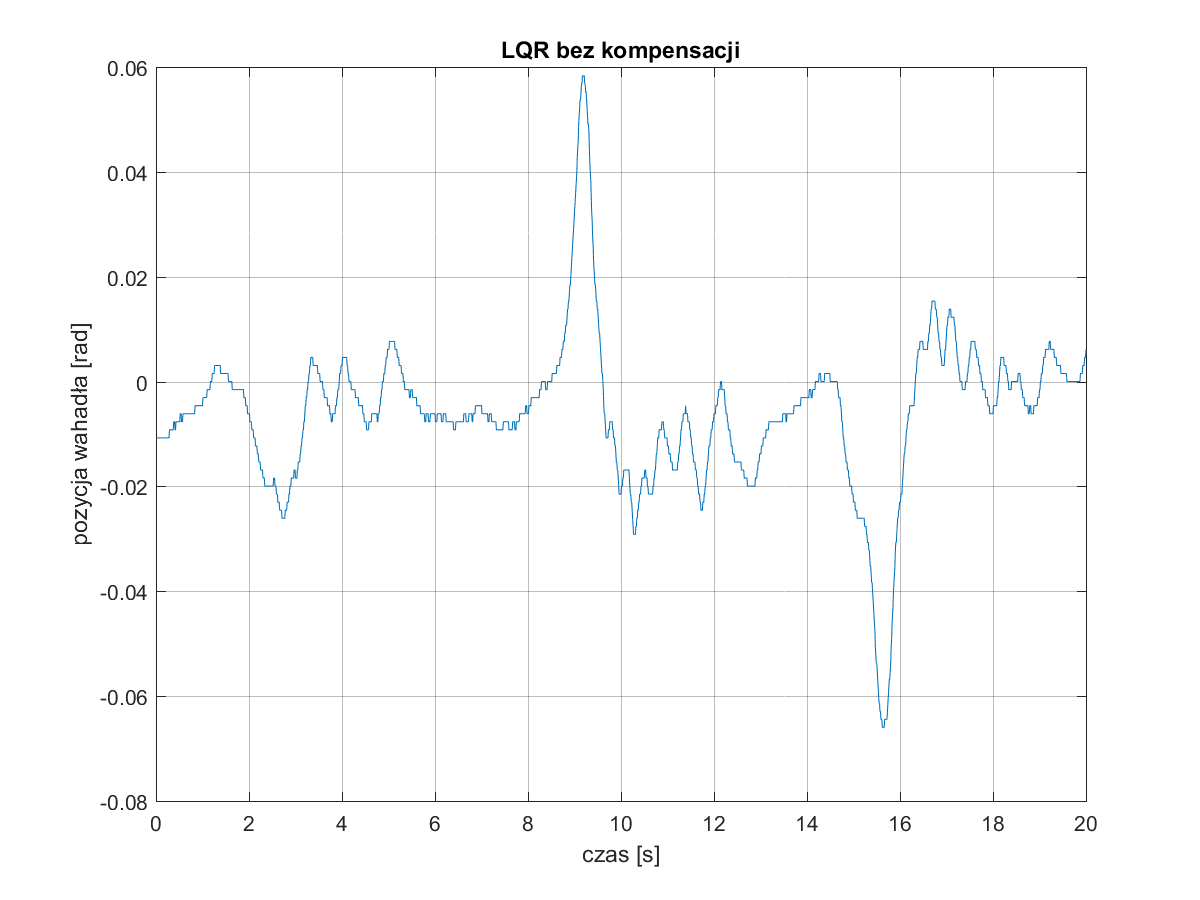
\includegraphics[width=3in]{obrazy/pendulum/LQR_bezk_poz_wah.png}}
	~~
	\subfloat{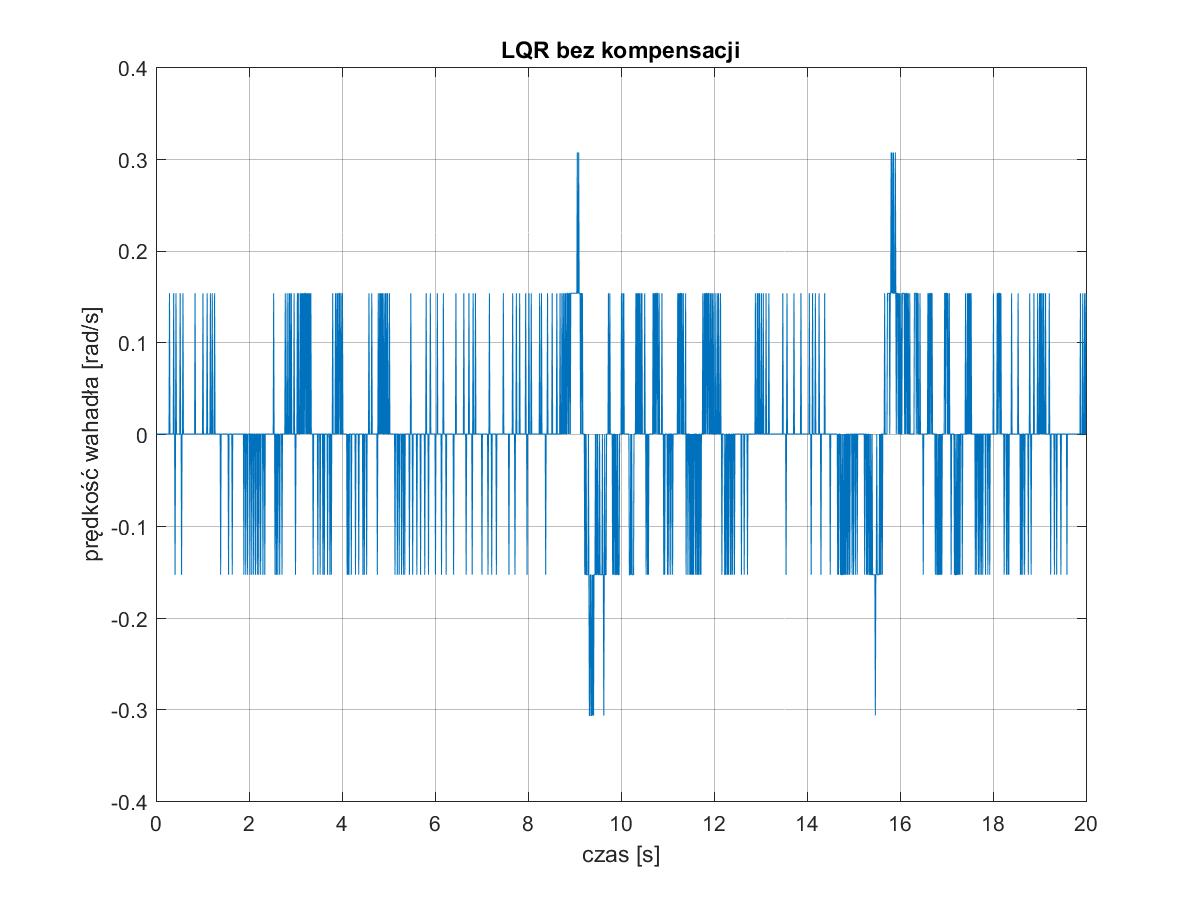
\includegraphics[width=3in]{obrazy/pendulum/LQR_bezk_pred_wah.png}}
	
	\subfloat{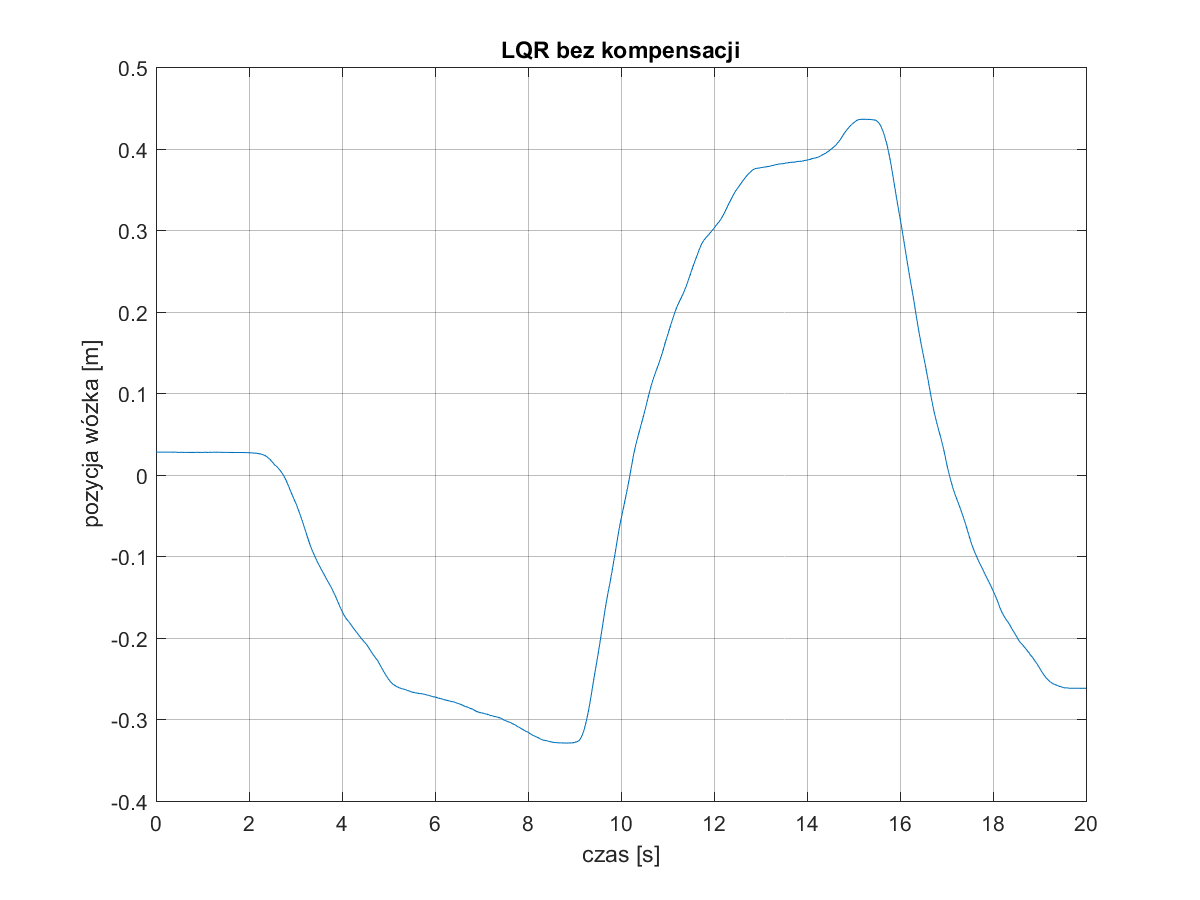
\includegraphics[width=3in]{obrazy/pendulum/LQR_bezk_poz_woz.png}}
	~~
	\subfloat{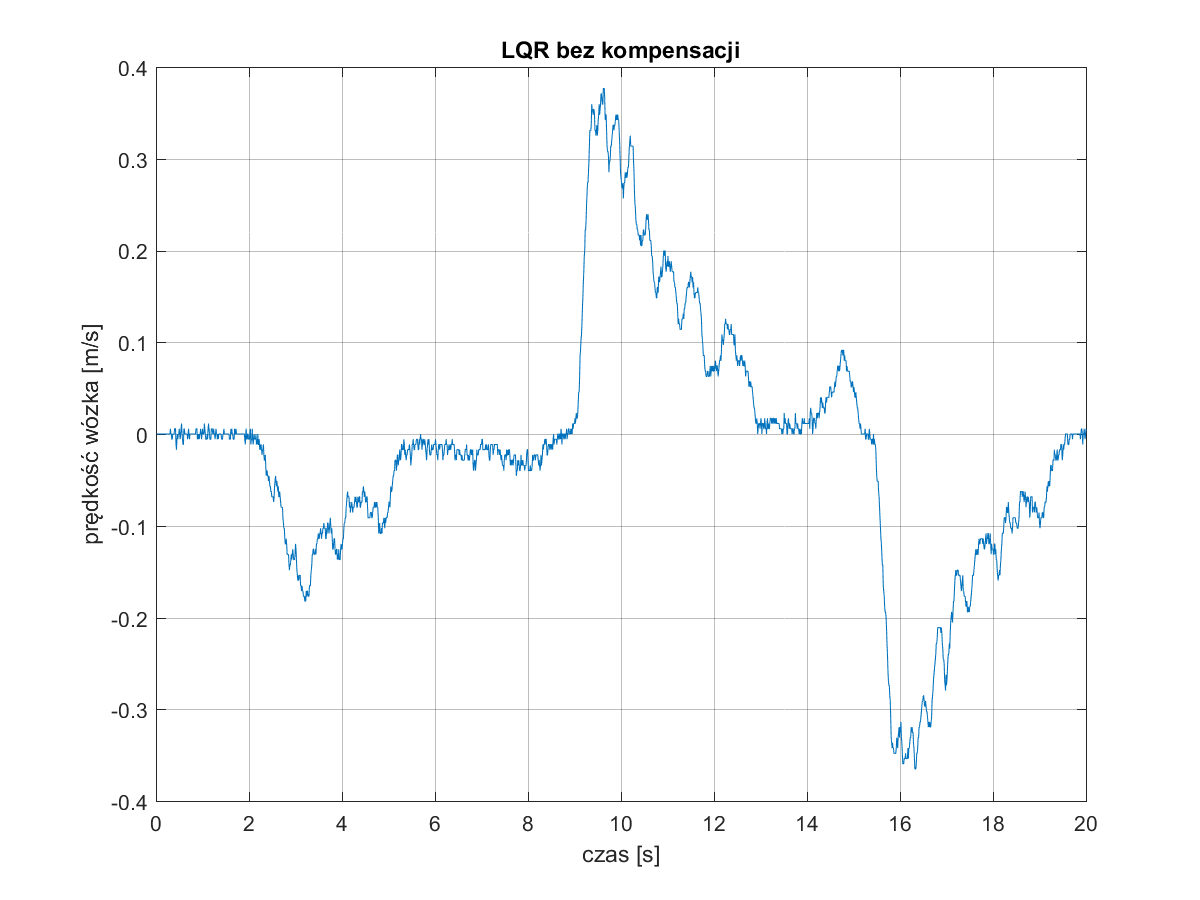
\includegraphics[width=3in]{obrazy/pendulum/LQR_bezk_pred_woz.png}}
	
	\subfloat{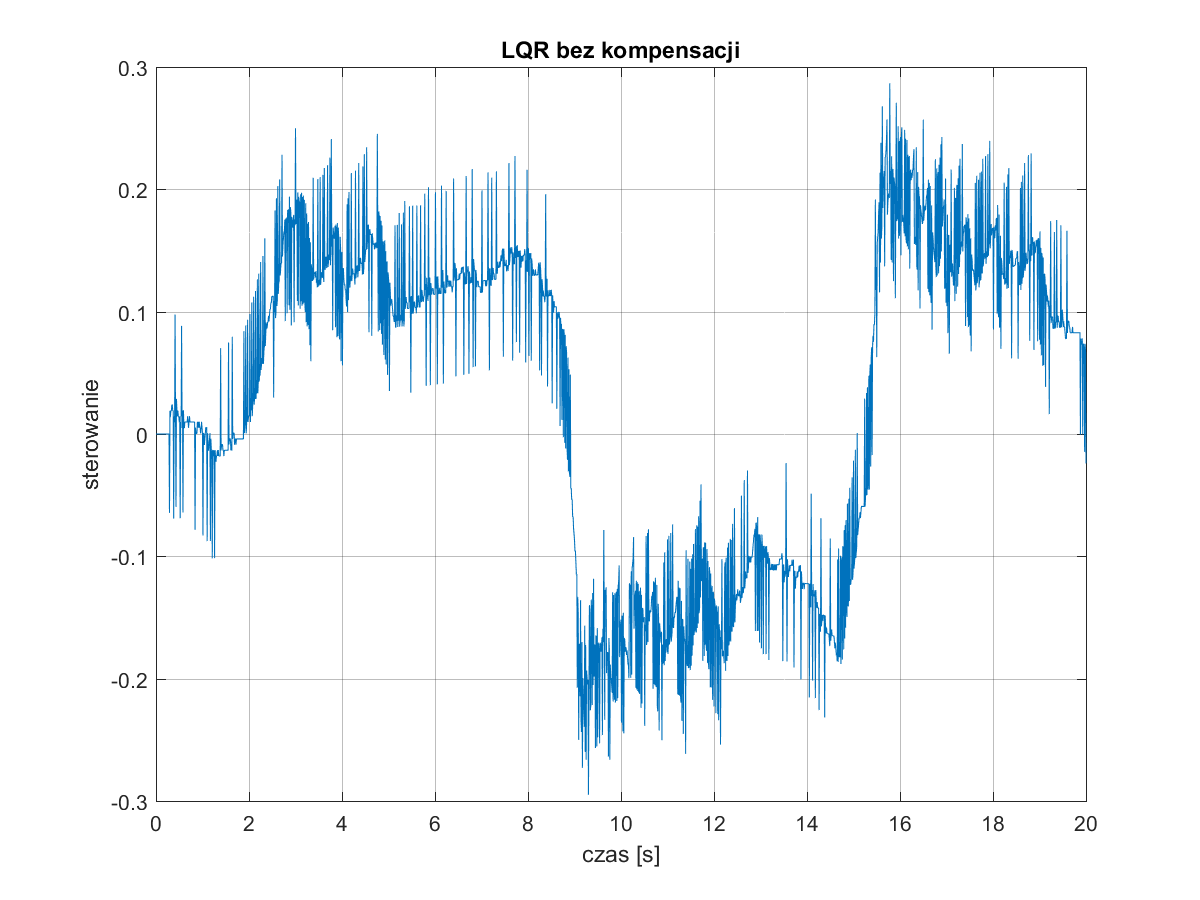
\includegraphics[width=3in]{obrazy/pendulum/LQR_bezk_ster.png}}
%	~~
%	\subfloat{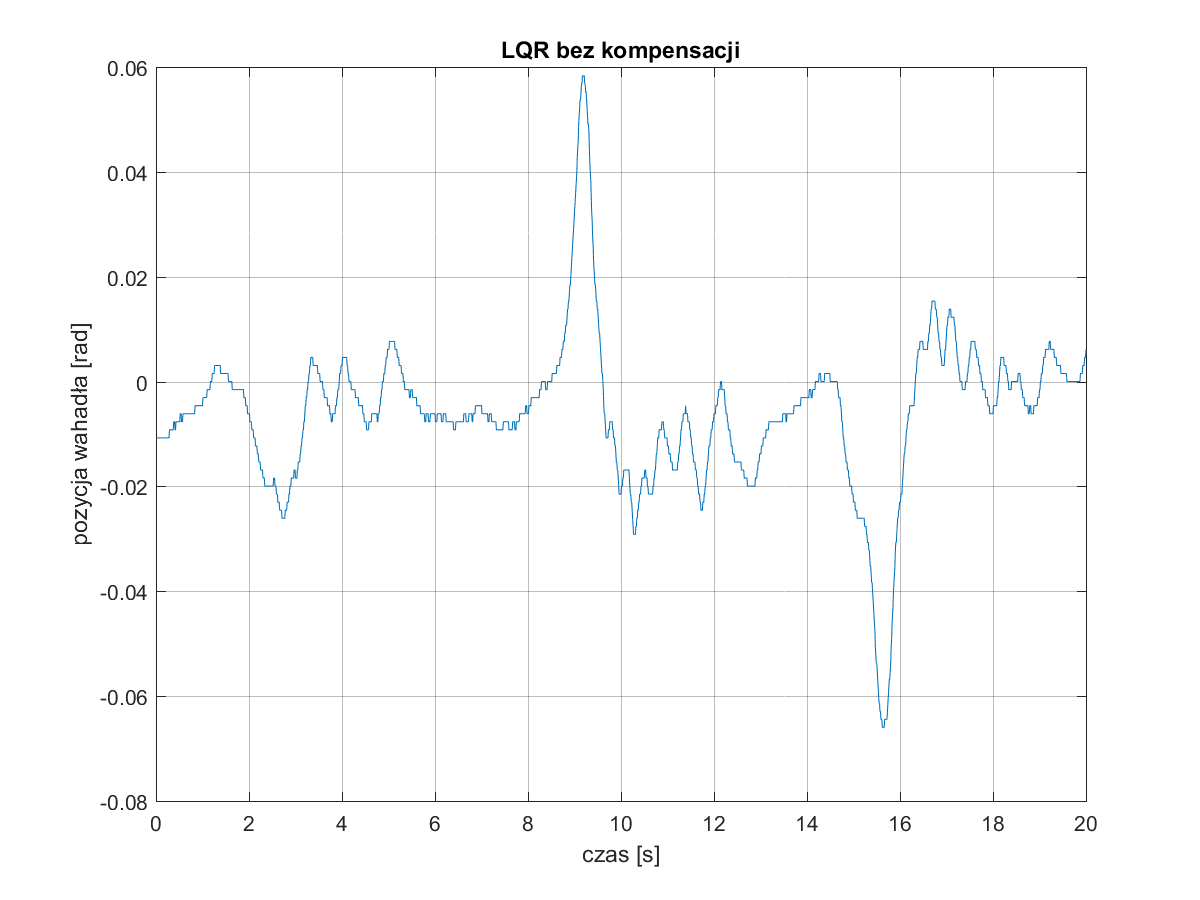
\includegraphics[width=2.8in]{obrazy/pendulum/LQR_bezk_poz_wah.png}}
	\caption{Zadanie stabilizacji obiektu w niestabilnym punkcie równowagi przy użyciu regulatora LQR bez kompensacji tarcia statycznego.}
\label{fig:LQRbezKom}
\end{figure}

Zauważono wpływ tarcia statycznego objawiający się oscylacjami wokół zadanego położenia wózka na szynie.
\subsection{Tarcie statyczne}
Modelowanie tarcia statycznego nie jest prostym zadaniem. Zaobserwowano, że napięcie podawane na silnik potrzebne do pokonania siły tarcia wózka o szynę nie jest stałe, zależy od położenia wózka. Aby zredukować niekorzystny wpływ tarcia na działanie systemu postanowiono wykorzystać następujące podejście. Sterowanie \ref{eq:u} wyliczone przez regulator zostanie zwiększone (w sensie wartości bezwzględnej) o stałą wartość kompensującą siłę tarcia $u_{F_T}=0.11$, która wyznaczona została eksperymentalnie:
\begin{equation}
\label{eq:Kompen}
u(t) = -(Kx(t)+u_{F_T}\cdot sgn(Kx(t))
\end{equation}
\begin{figure}[H]
	\centering
	\subfloat{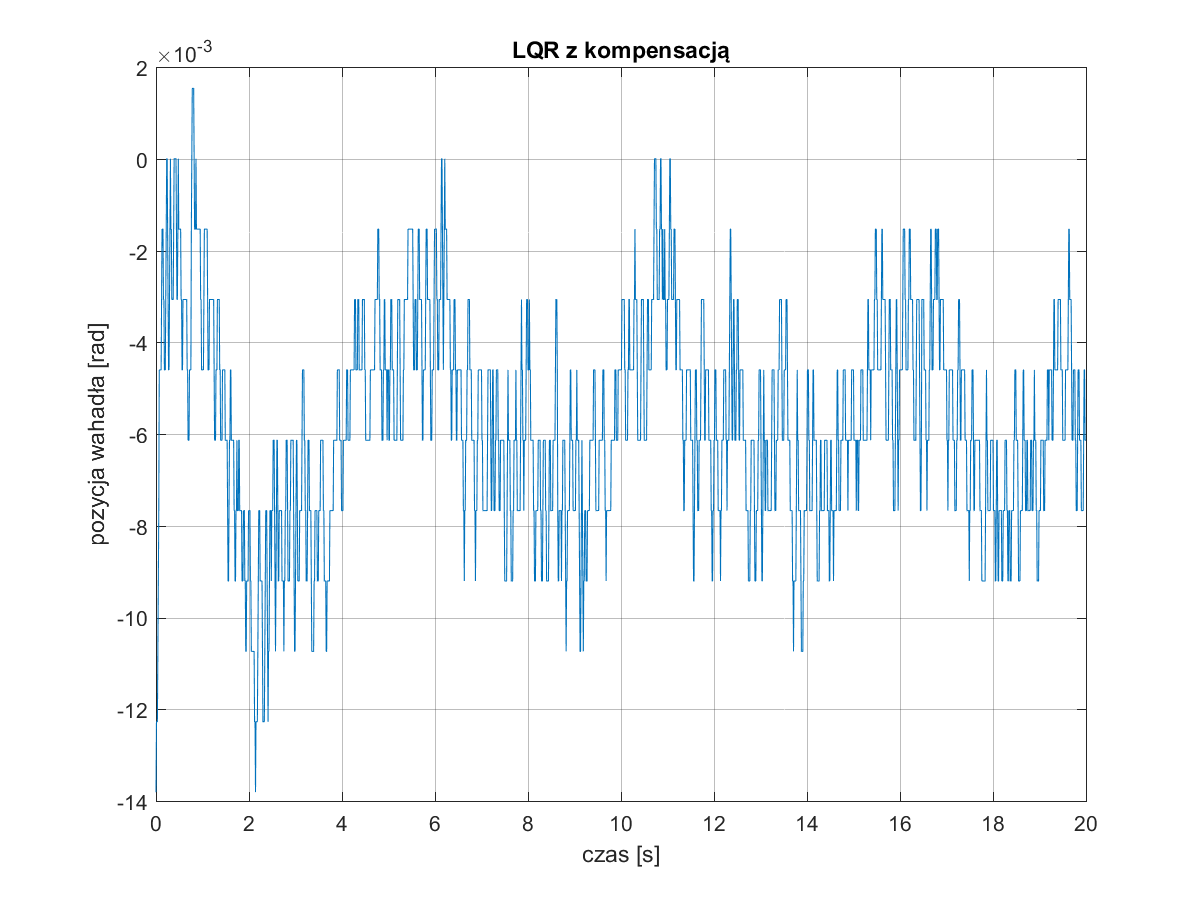
\includegraphics[width=3in]{obrazy/pendulum/LQR_zk_poz_wah.png}}
	~~
	\subfloat{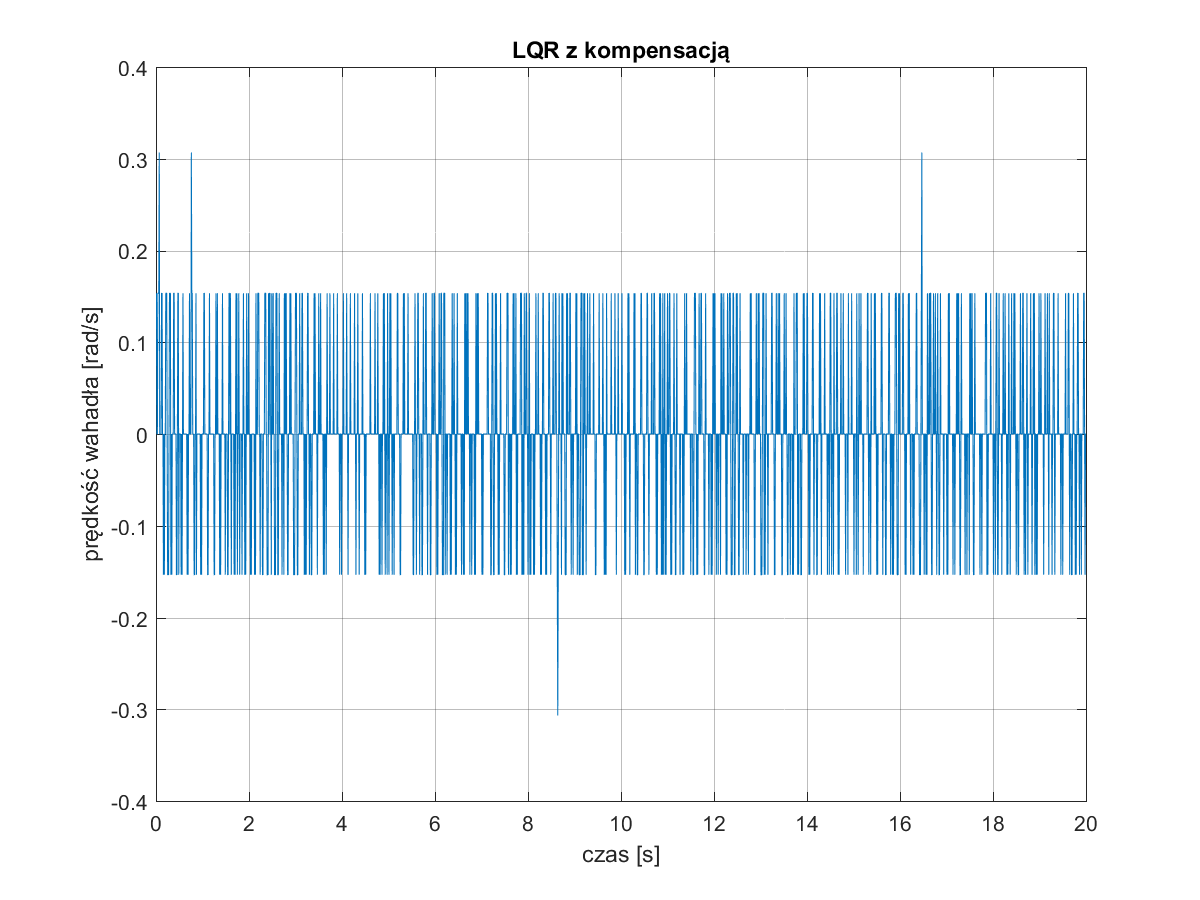
\includegraphics[width=3in]{obrazy/pendulum/LQR_zk_pred_wah.png}}
	
	\subfloat{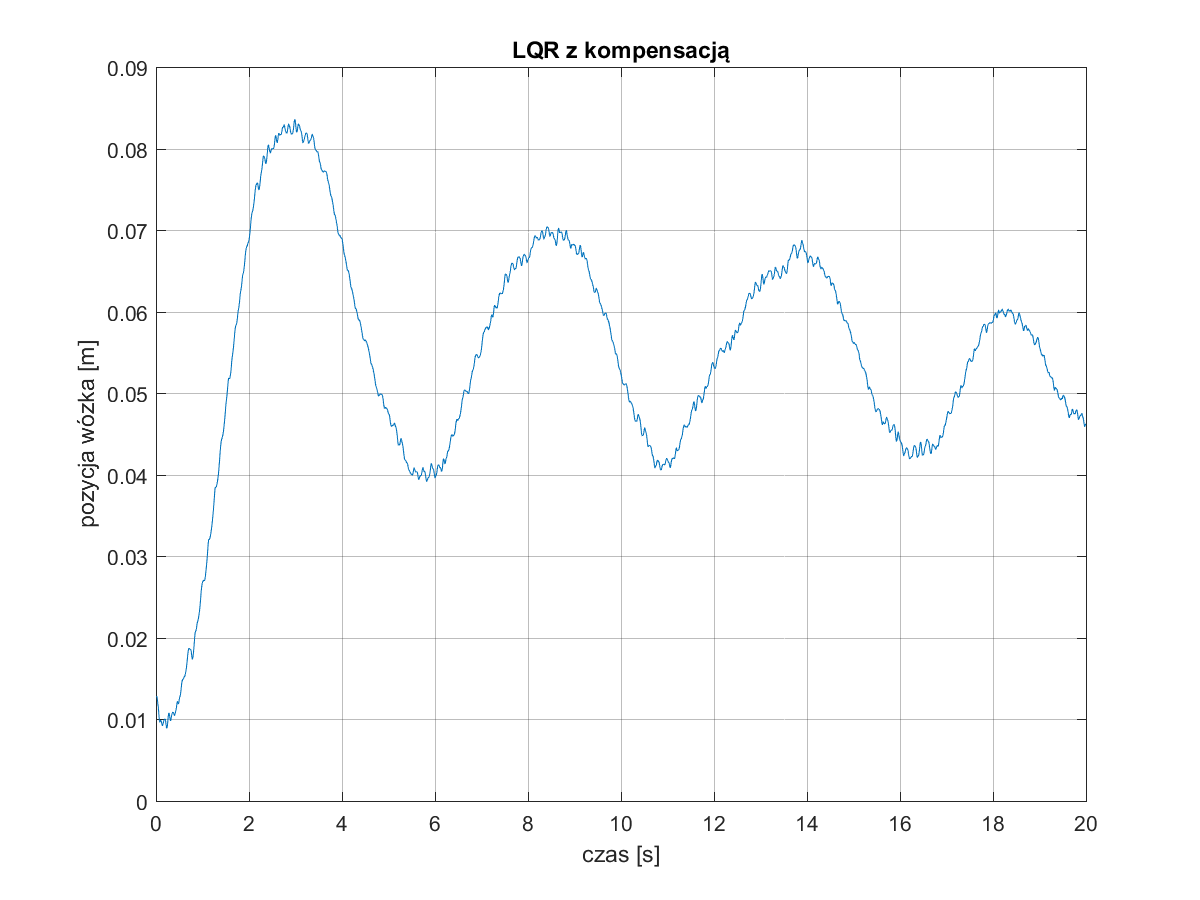
\includegraphics[width=3in]{obrazy/pendulum/LQR_zk_poz_woz.png}}
	~~
	\subfloat{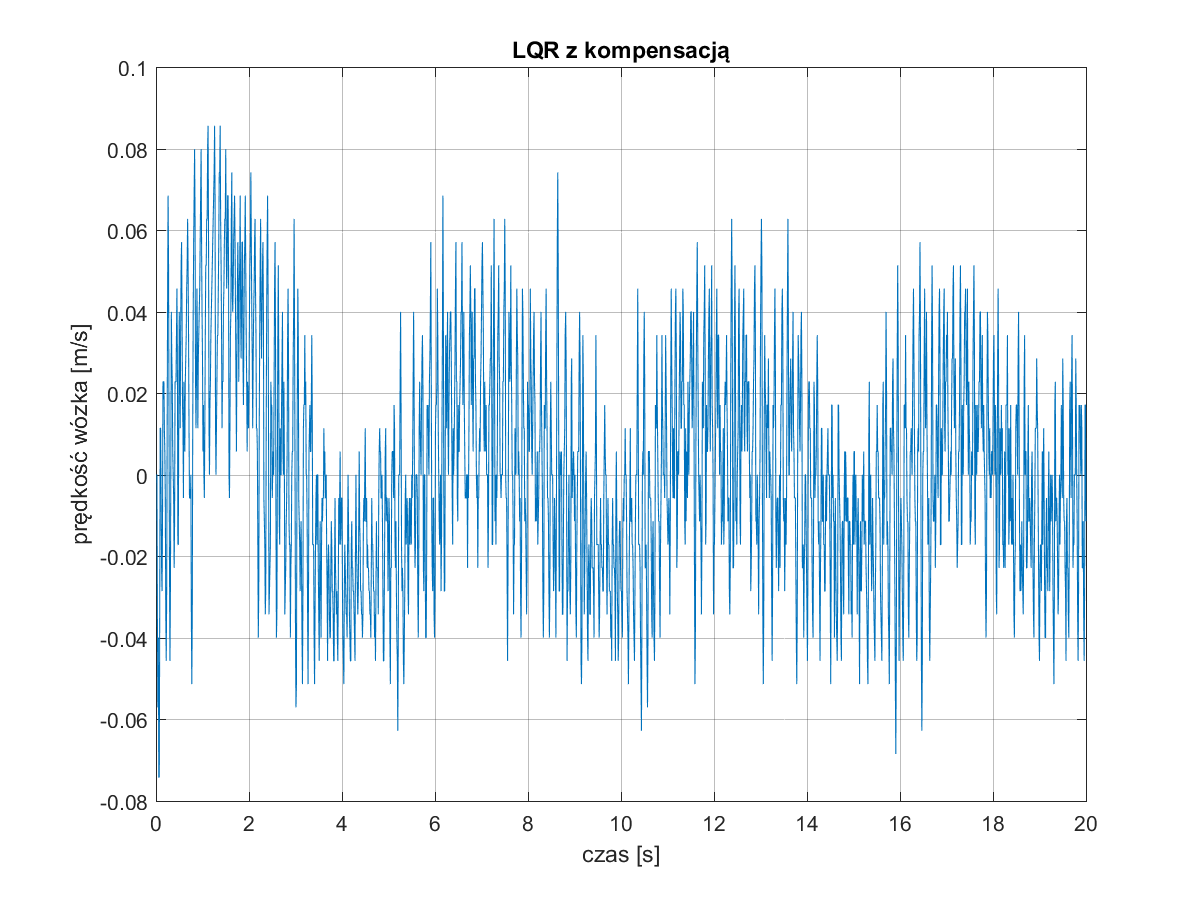
\includegraphics[width=3in]{obrazy/pendulum/LQR_zk_pred_woz.png}}
	
	\subfloat{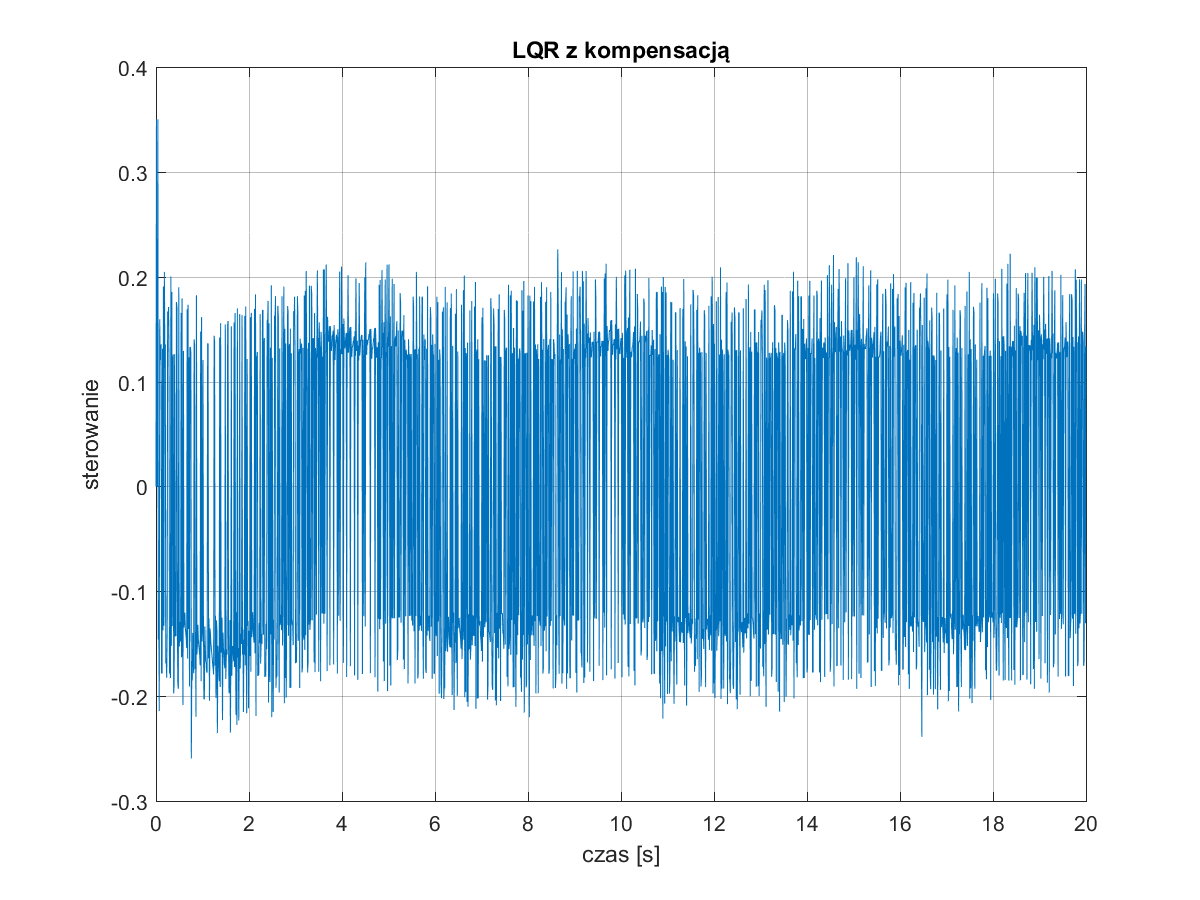
\includegraphics[width=3in]{obrazy/pendulum/LQR_zk_ster.png}}
%	~~
%	\subfloat{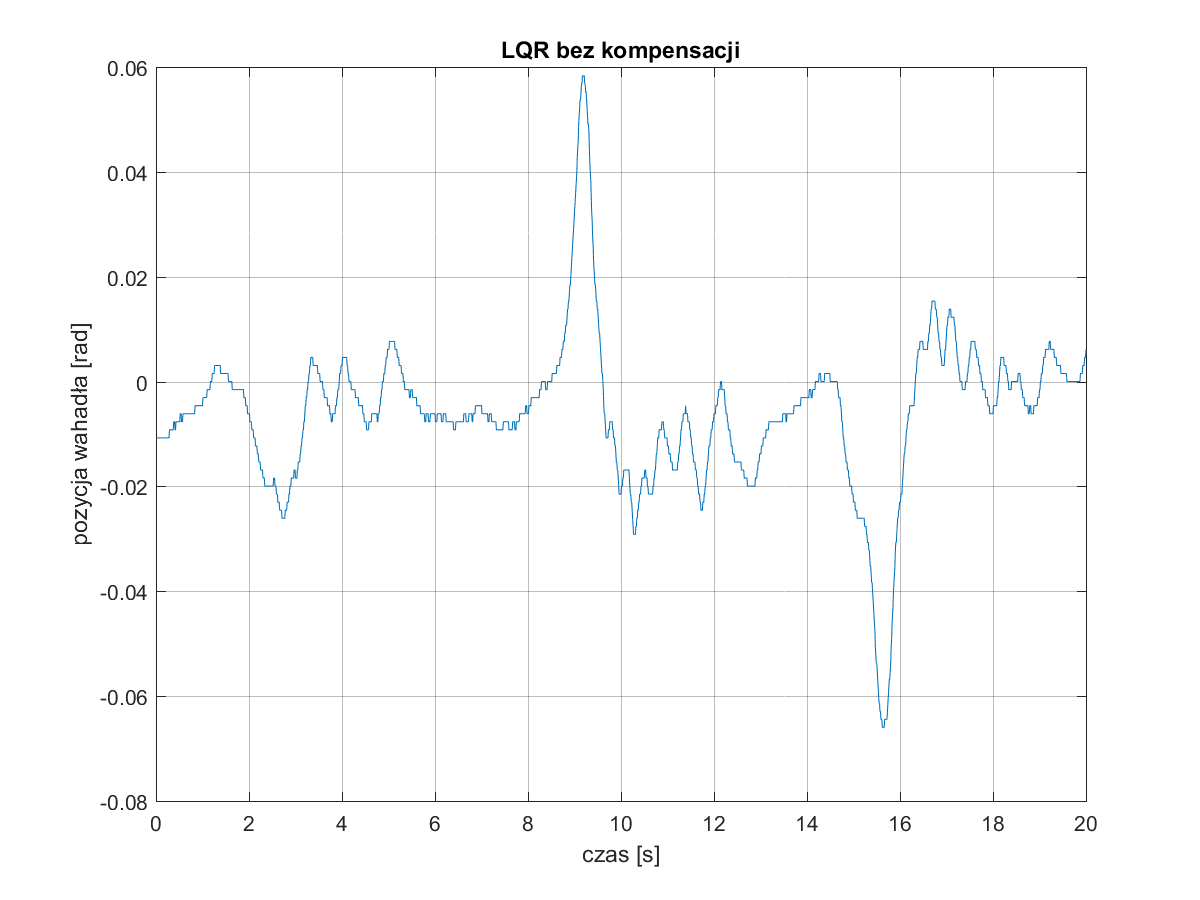
\includegraphics[width=2.8in]{obrazy/pendulum/LQR_bezk_poz_wah.png}}
	\caption{Zadanie stabilizacji obiektu w niestabilnym punkcie równowagi przy użyciu regulatora LQR z kompensacją tarcia statycznego.}
\label{fig:LQRkom}
\end{figure}
Problem oscylacji wózka został w znaczącym stopniu zażegnany. Amplituda wychyleń wózka zmalała blisko dziesięciokrotnie co ukazane zostało na rysunkach \ref{fig:LQRbezKom} oraz \ref{fig:LQRkom}. Zastosowanie regulatora opisanego równaniem \ref{eq:Kompen}  wprowadziło nieciągłości funkcji sterującej w punktach:
 \begin{equation}
\left\lbrace x: Kx(t)=0\right\rbrace 
\end{equation}
Nieciągłości te objawiały się widocznymi drganiami wózka o wysokiej częstotliwości.
% wykres drgań

\section{Obserwator stanu}
\subsection{Obserwator Luenbergera}
Po szczegółowej analizie zarejestrowanych przebiegów zauważono duży wpływ szumu kwantyzacji na jakość regulacji, szczególnie w przypadku prędkości kątowej wahadła wyliczanej przez iloraz różnicowy położenia wahadła w kolejnych chwilach czasu. W celu wygładzenia przebiegu prędkości zaprojektowano obserwator Luenbergera dla systemu zlinearyzowanego w taki sposób, aby błąd estymacji prędkości dostatecznie szybko zdążał do zera. Doświadczalnie wyznaczono odpowiednie ujemne wartości własne macierzy:
\begin{equation}  
eig(A-LC) = \left\lbrace wartosci dopisac \right\rbrace 
\end{equation} 
Zdecydowano się na obserwator pełnego rzędu, natomiast do regulatora podano jedynie estymacje stanów obarczonych największym błędem pomiarowym - prędkości wahadła i wózka.
% przebiegi porównawcze

\subsection{Model ARMAX}

\section{Regulator \textit{swing-up}}
\subsection{Algorytm \textit{swing-up}}
Zastosowano heurystyczną regułę, która w zależności od położenia i prędkości wahadła pozwala wyznaczyć sterowanie wzbudzające system:
\begin{equation}  
u(t) = u_{swing}\cdot sgn[x_2(|x_1|-\frac{\pi}{2})]
\end{equation} 
gdzie amplituda sygnału sterującego $u_{swing} = 0.3$ wyznaczona została eksperymentalnie, tak aby położenie wózka podczas rozhuśtywania wahadła nie wykroczyło poza dopuszczalne granice. 
\subsection{Warunek przełączenia}
Algorytm \textit{swing-up} realizowany jest do momentu, kiedy do systemu zostanie dostarczona odpowiednia ilość energii, aby doprowadzić wahadło w okolice niestabilnego położenia równowagi.
Następnie sterowanie zostaje całkowicie odłączone do momentu, kiedy położenie wahadła znajdzie się w granicach $(-10^\circ,10^\circ)$. Wtedy zostaje aktywowany regulator LQR. W przypadku, kiedy stabilizacja nie powiedzie się, kąt wahadła osiągnie wartość spoza zbioru $(-30^\circ,30^\circ)$ aktywowany na nowo zostaje algorytm \textit{swing-up}. Algorytm zrealizowany został na przerzutniku RS.
\begin{figure}[H]
	\centering
	\subfloat{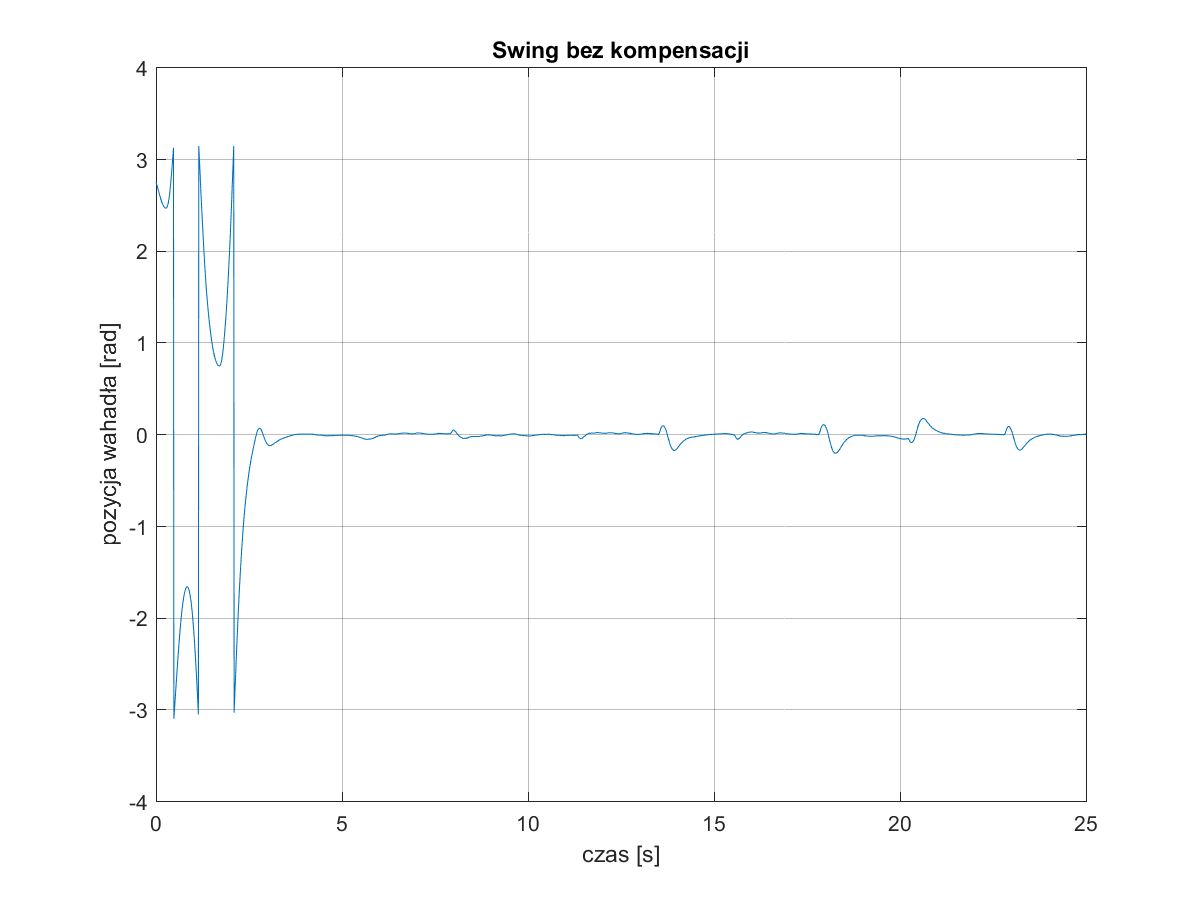
\includegraphics[width=3in]{obrazy/pendulum/Swing_bez_komp_poz_wah.png}}
	~~
	\subfloat{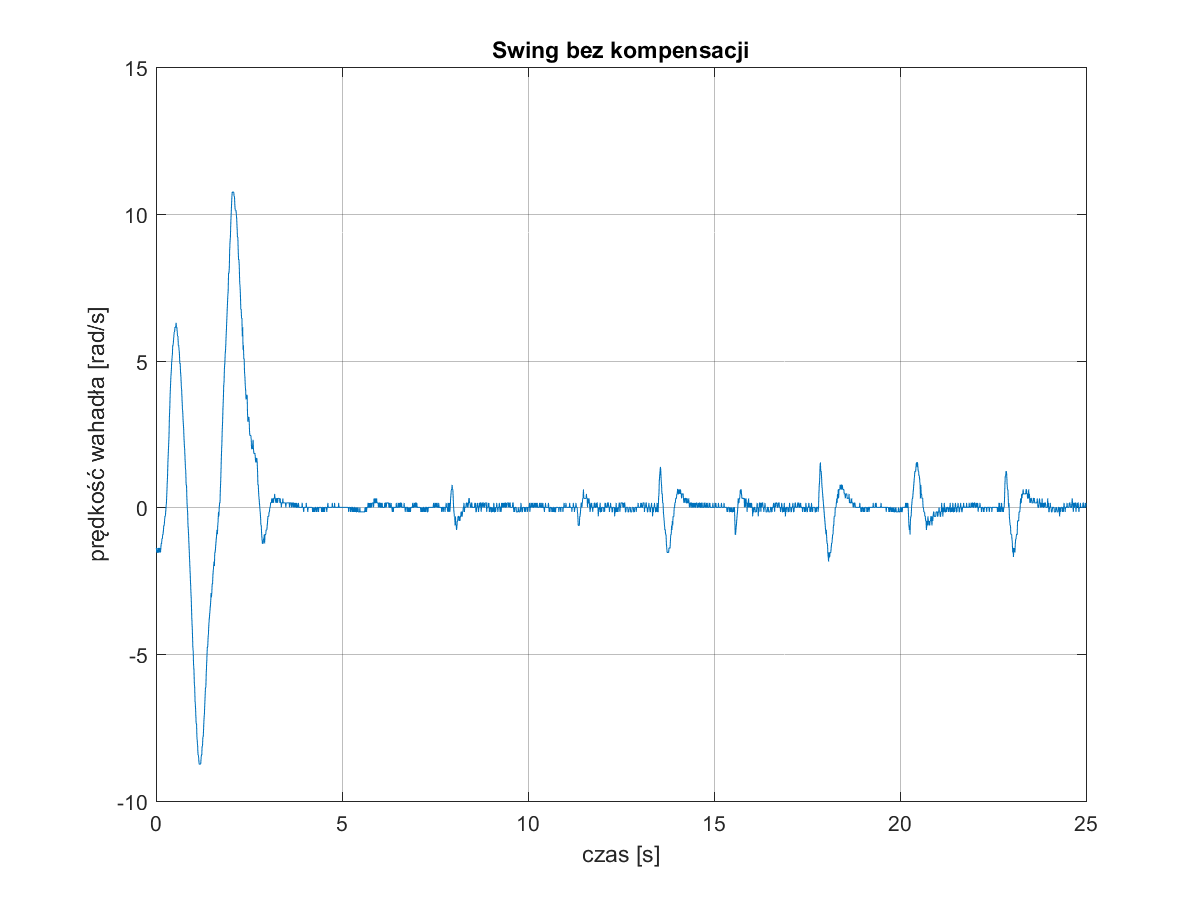
\includegraphics[width=3in]{obrazy/pendulum/Swing_bez_komp_pred_wah.png}}
	
	\subfloat{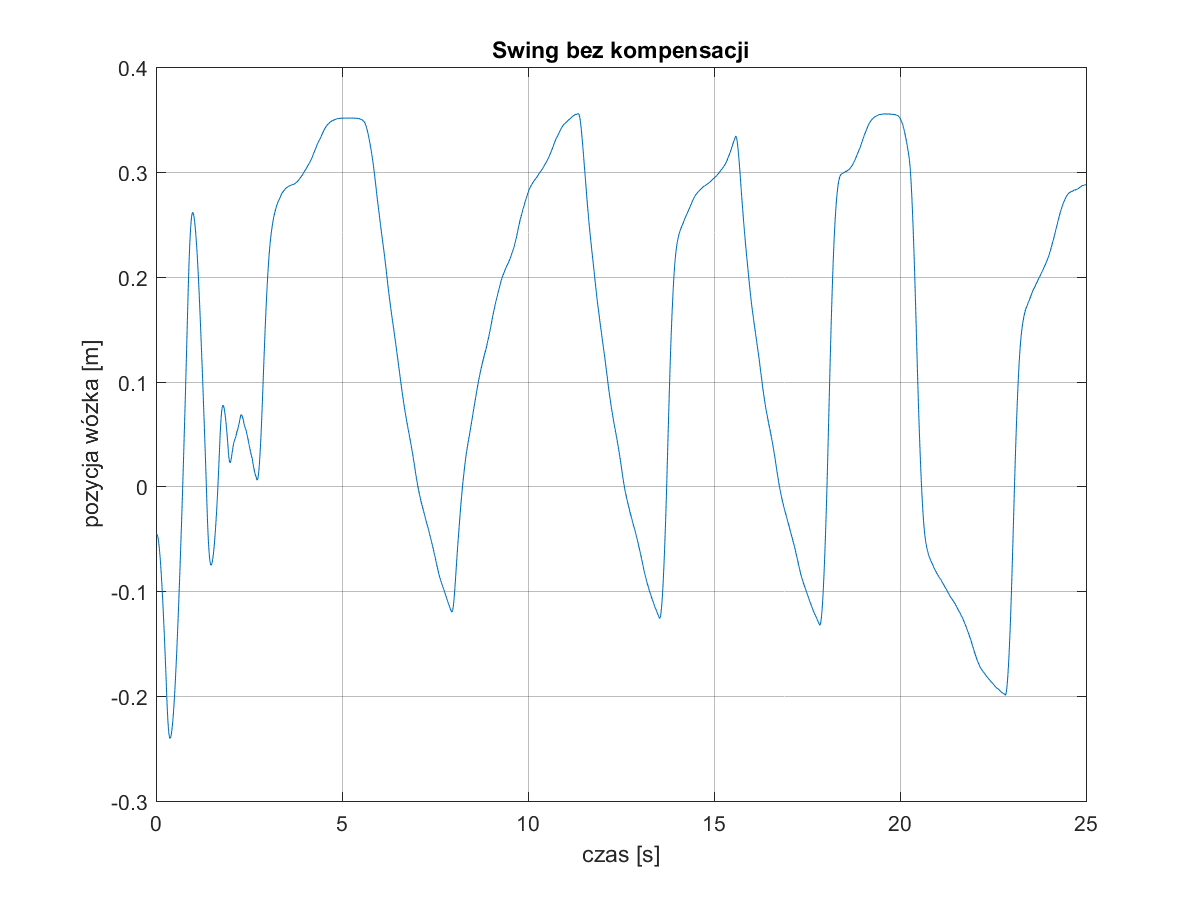
\includegraphics[width=3in]{obrazy/pendulum/Swing_bez_komp_poz_woz.png}}
	~~
	\subfloat{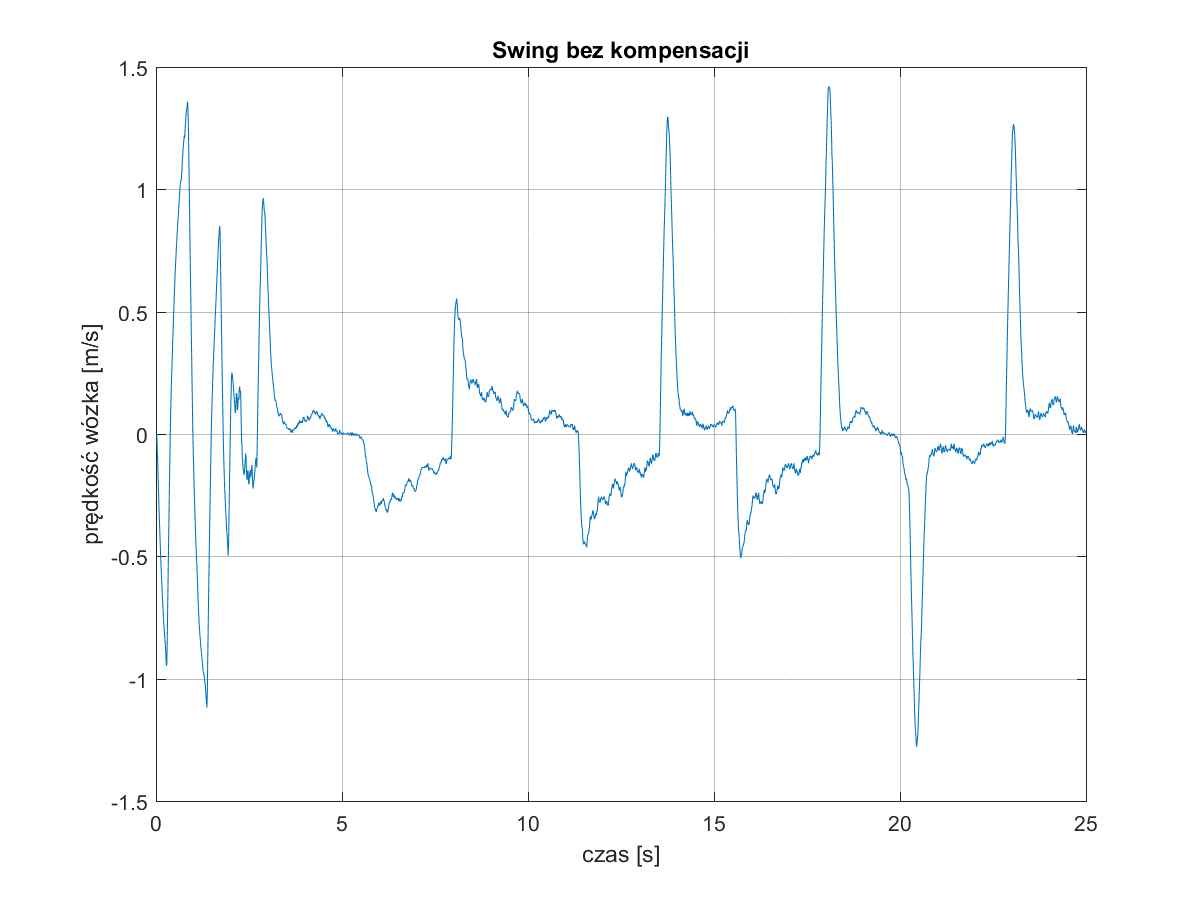
\includegraphics[width=3in]{obrazy/pendulum/Swing_bez_komp_pred_woz.png}}
	
	\subfloat{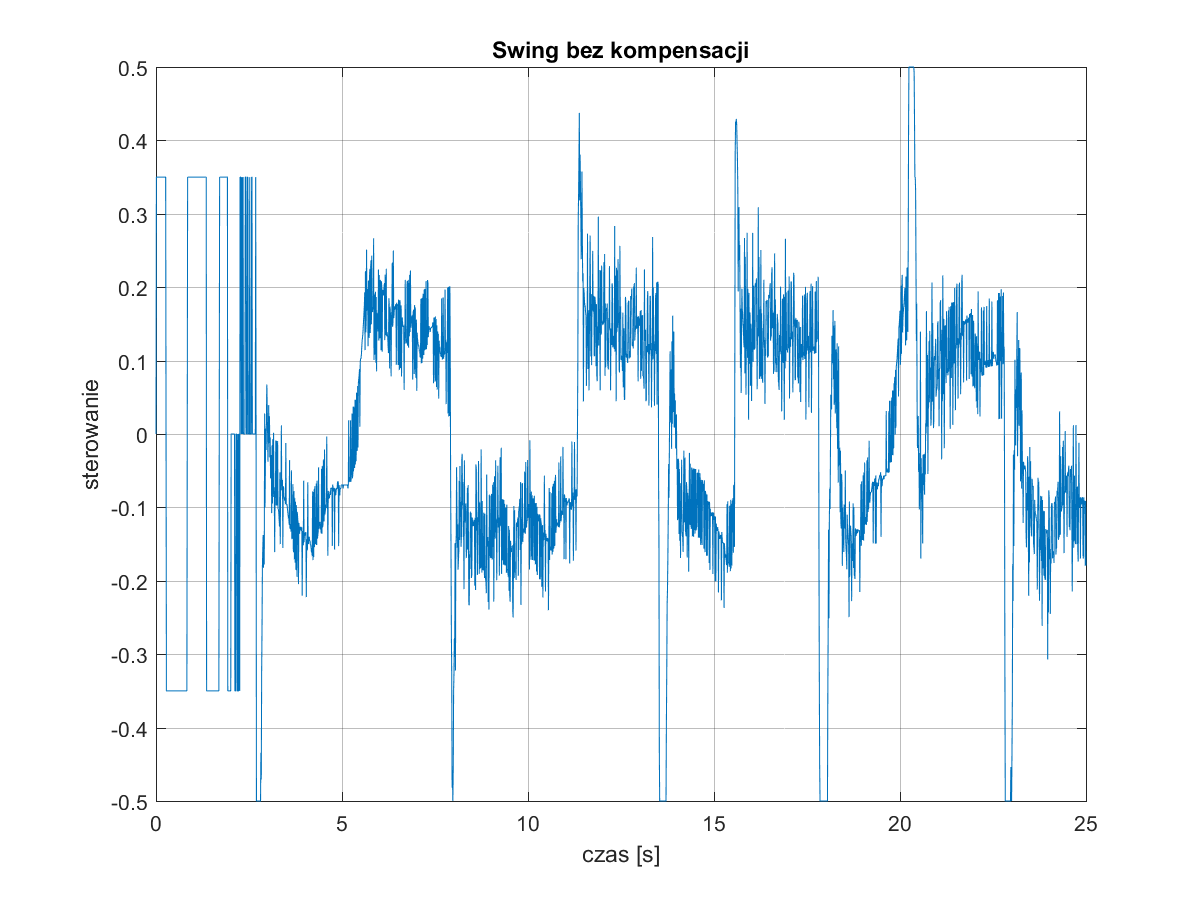
\includegraphics[width=3in]{obrazy/pendulum/Swing_bez_komp_ster.png}}
%	~~
%	\subfloat{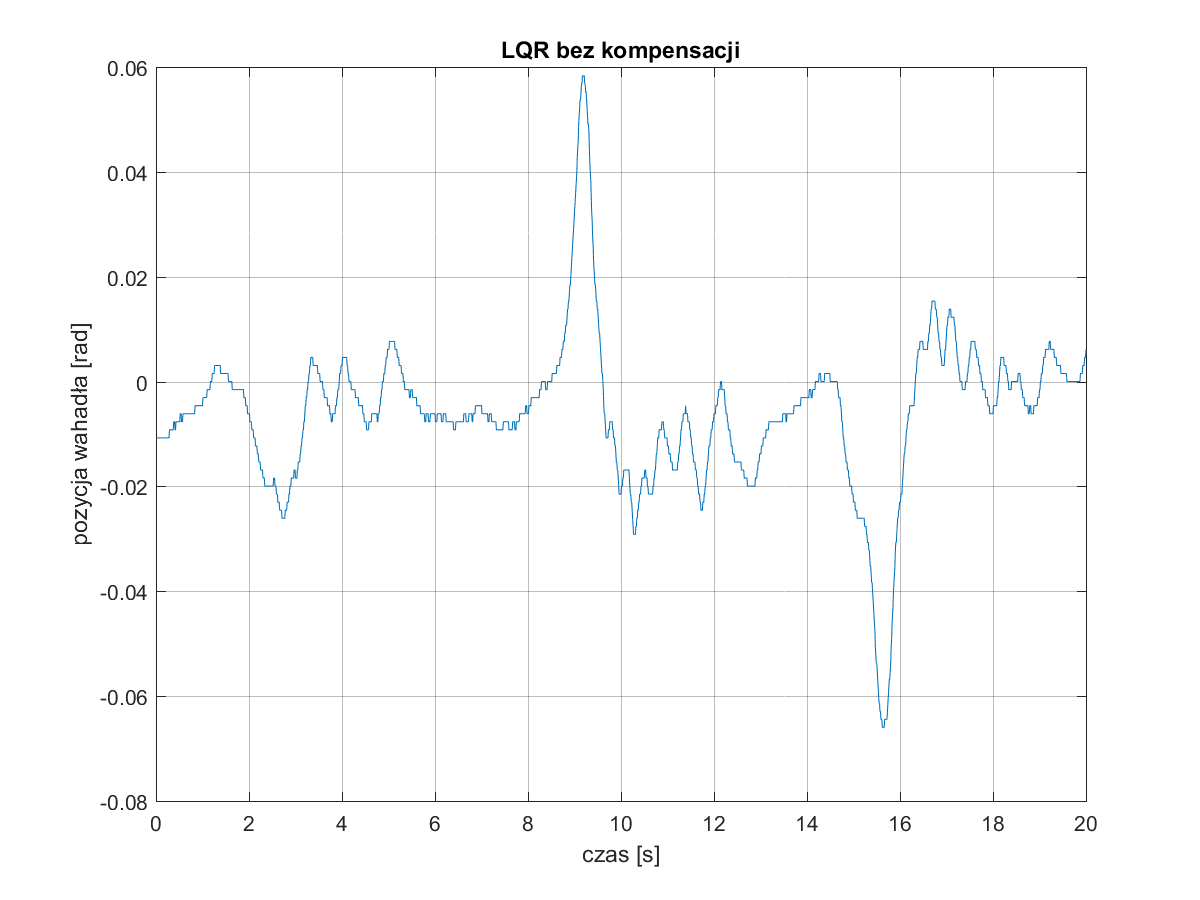
\includegraphics[width=2.8in]{obrazy/pendulum/LQR_bezk_poz_wah.png}}
	\caption{Swing-up wraz ze stabilizacją wahadła.}
\label{fig:Swing1}
\end{figure}
W celu zwiększenia skuteczności algorytmu, w momencie $t_p$ przełączania się na regulator LQR ustawiano punkt równowagi $x_0=[0,0,x_3(t_p),0]^T$. Po ustabilizowaniu się wahadła powracano do zerowego punktu równowagi. Warto odnotować, że kąt wahadła podczas skokowej zmiany wartości zadanej położenia wózka cały czas pozostawał bardzo blisko zera.
\begin{figure}[H]
	\centering
	\subfloat{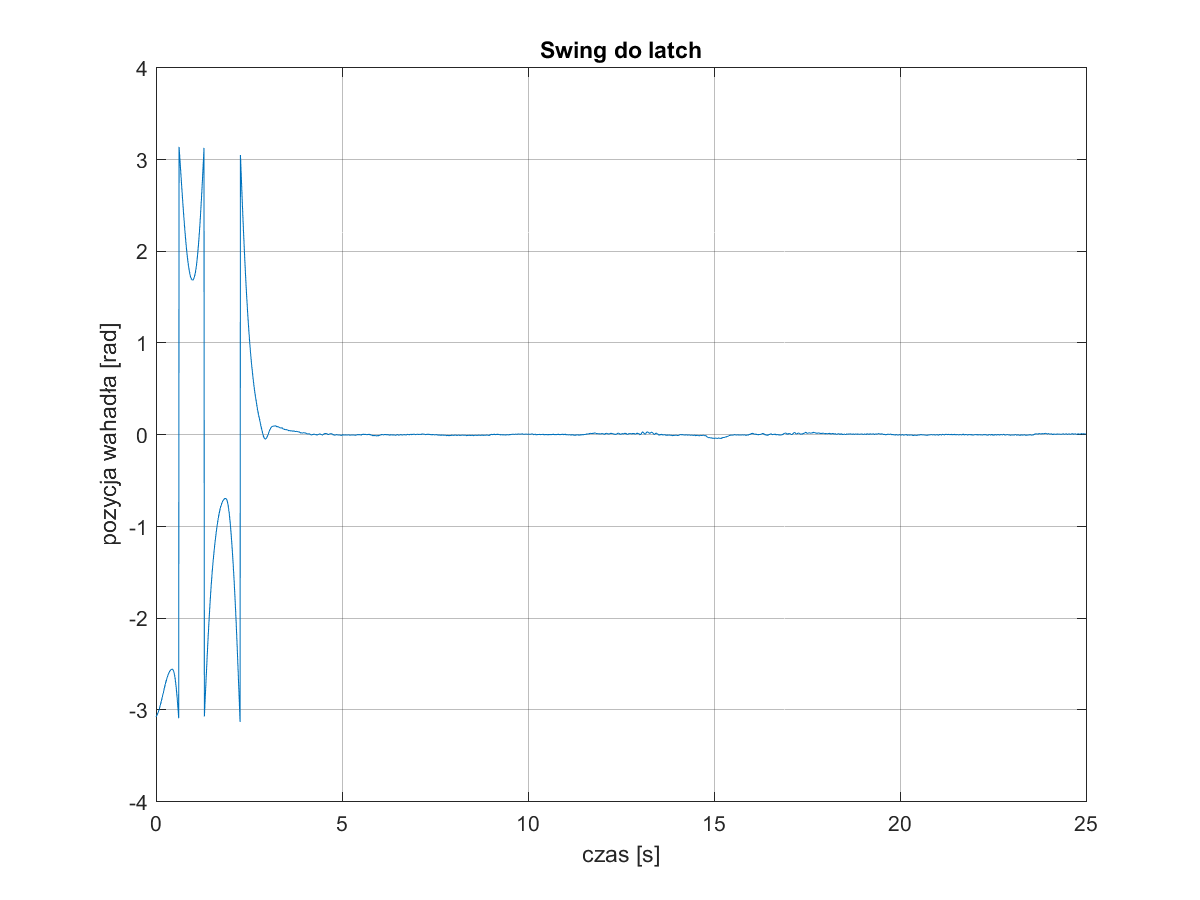
\includegraphics[width=3in]{obrazy/pendulum/Swing_do_latch_poz_wah.png}}
	~~
	\subfloat{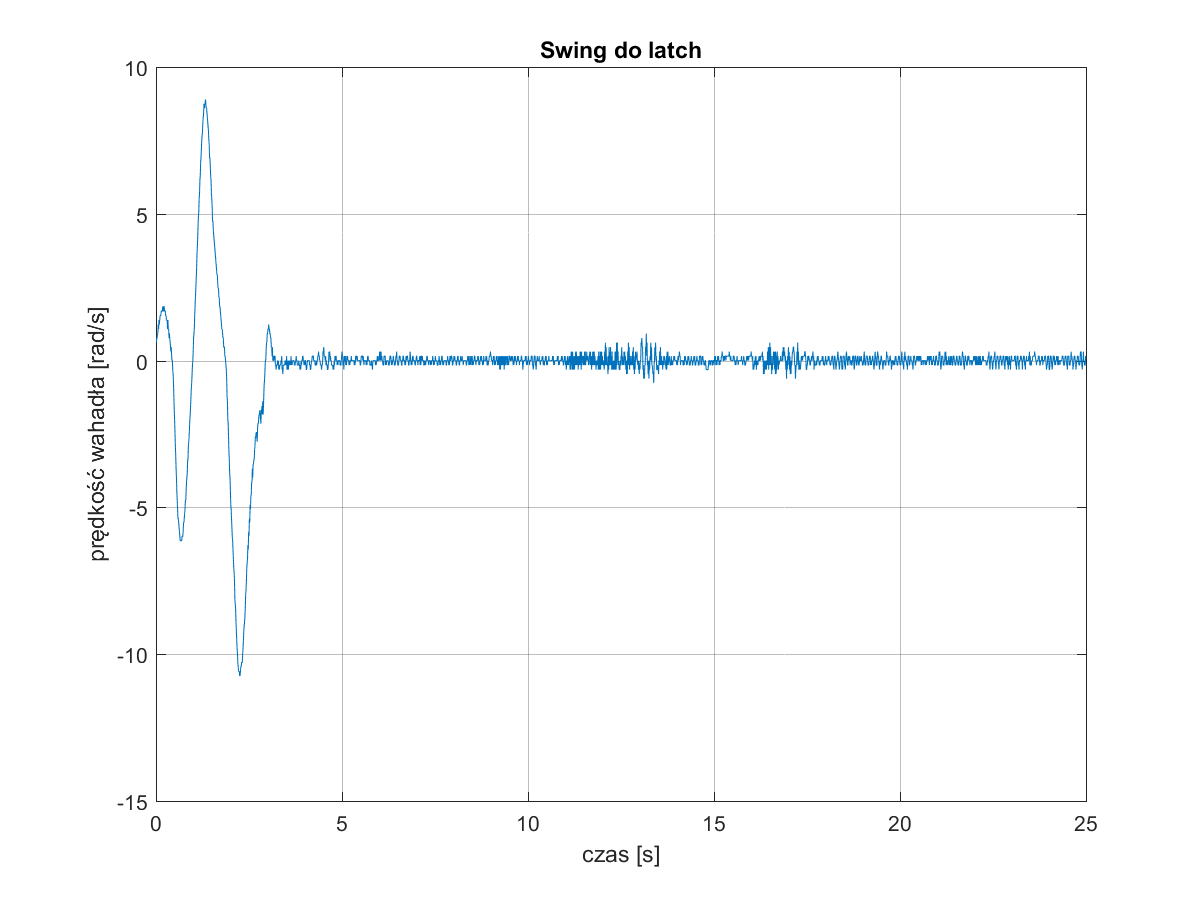
\includegraphics[width=3in]{obrazy/pendulum/Swing_do_latch_pred_wah.png}}
	
	\subfloat{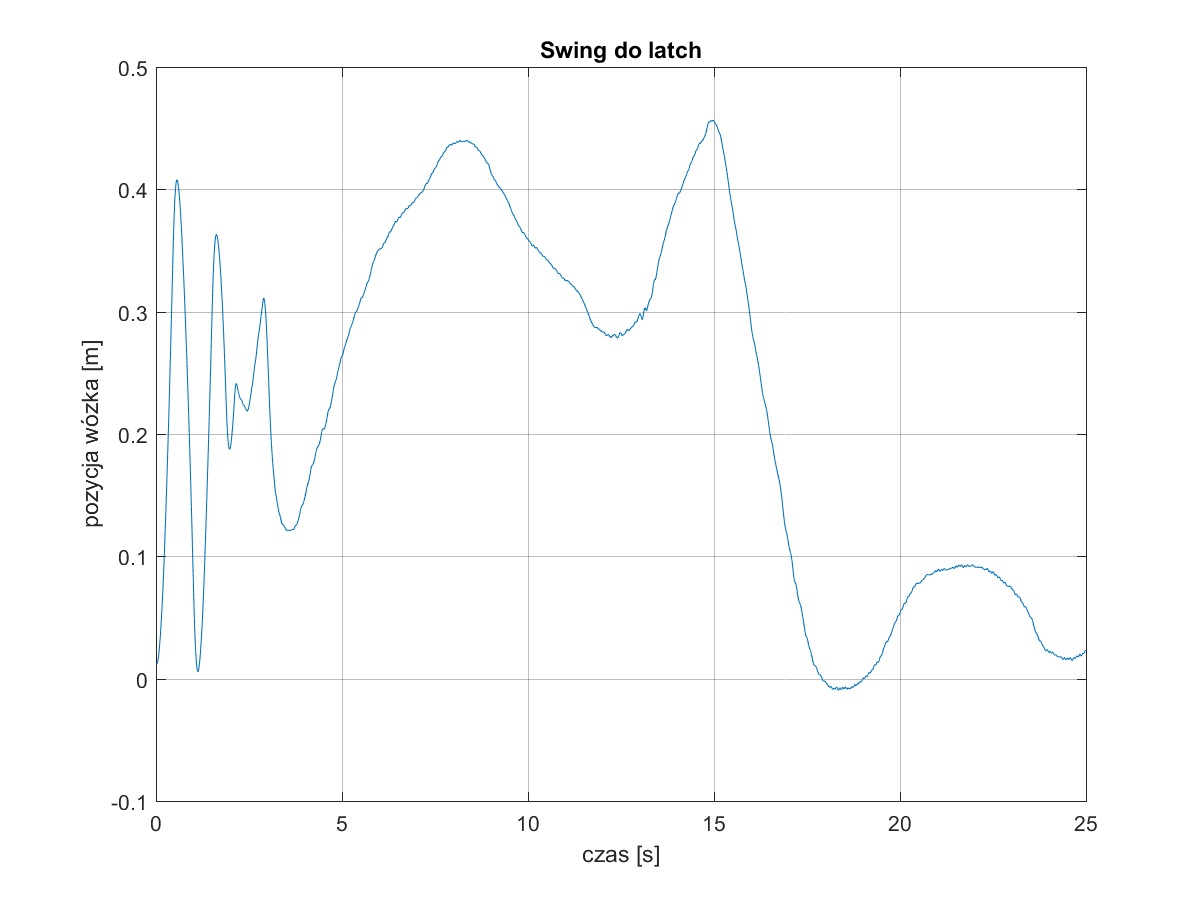
\includegraphics[width=3in]{obrazy/pendulum/Swing_do_latch_poz_woz.png}}
	~~
	\subfloat{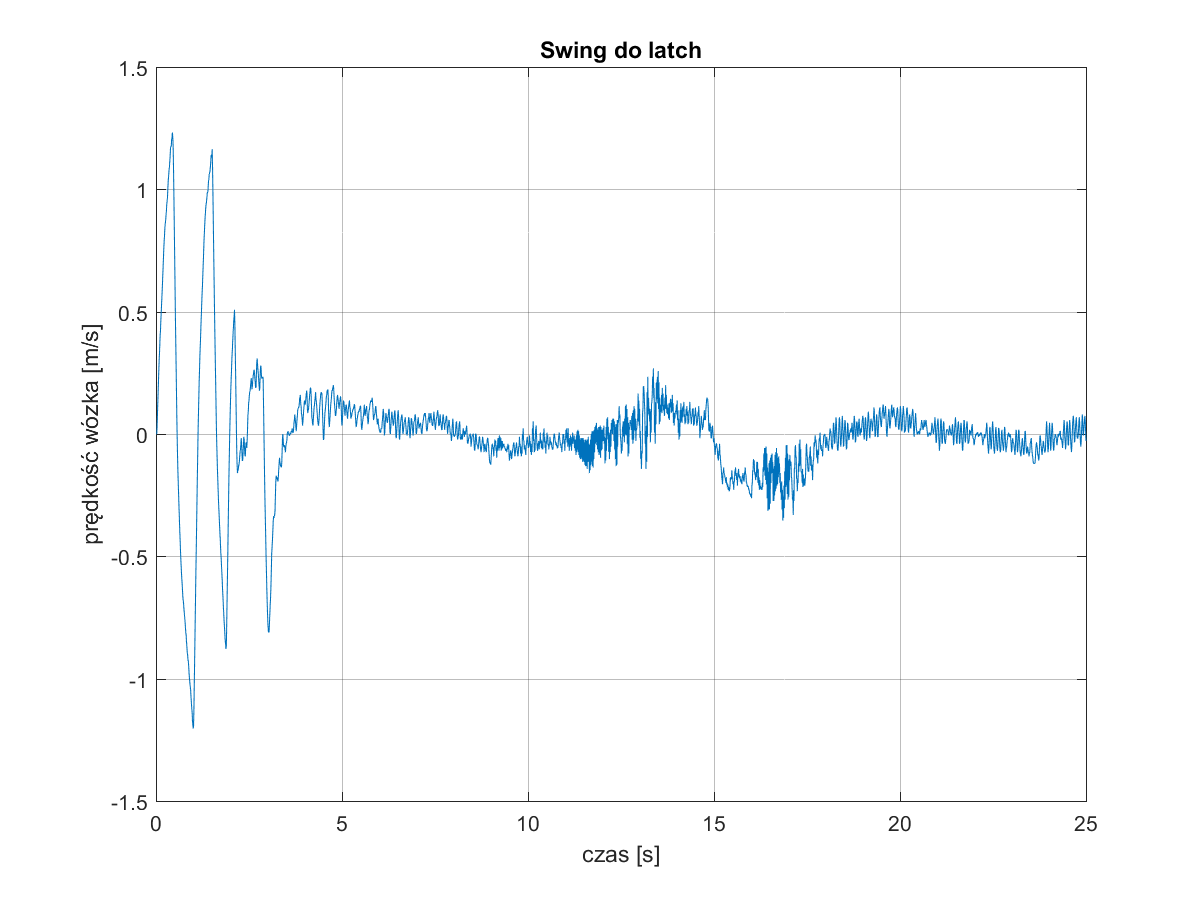
\includegraphics[width=3in]{obrazy/pendulum/Swing_do_latch_pred_woz.png}}
	
	\subfloat{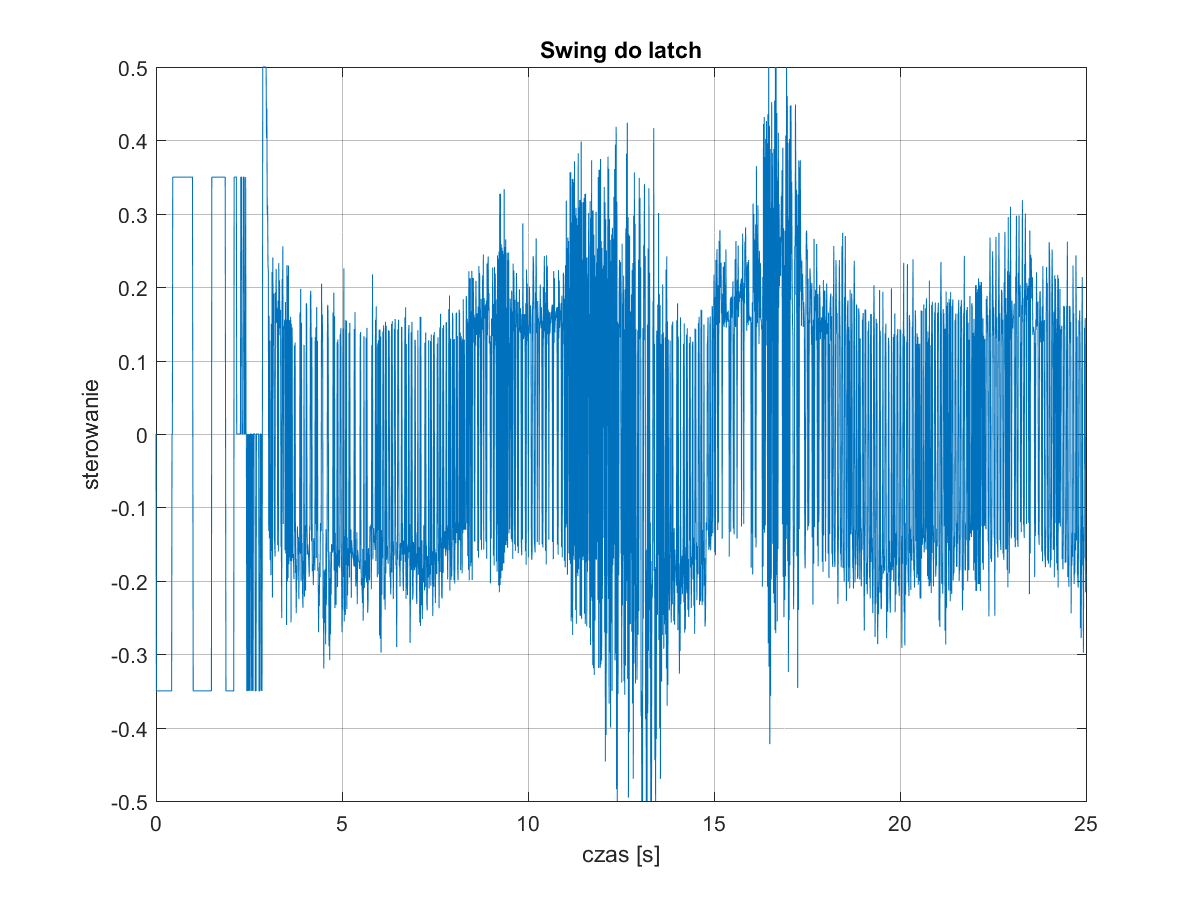
\includegraphics[width=3in]{obrazy/pendulum/Swing_do_latch_ster.png}}
%	~~
%	\subfloat{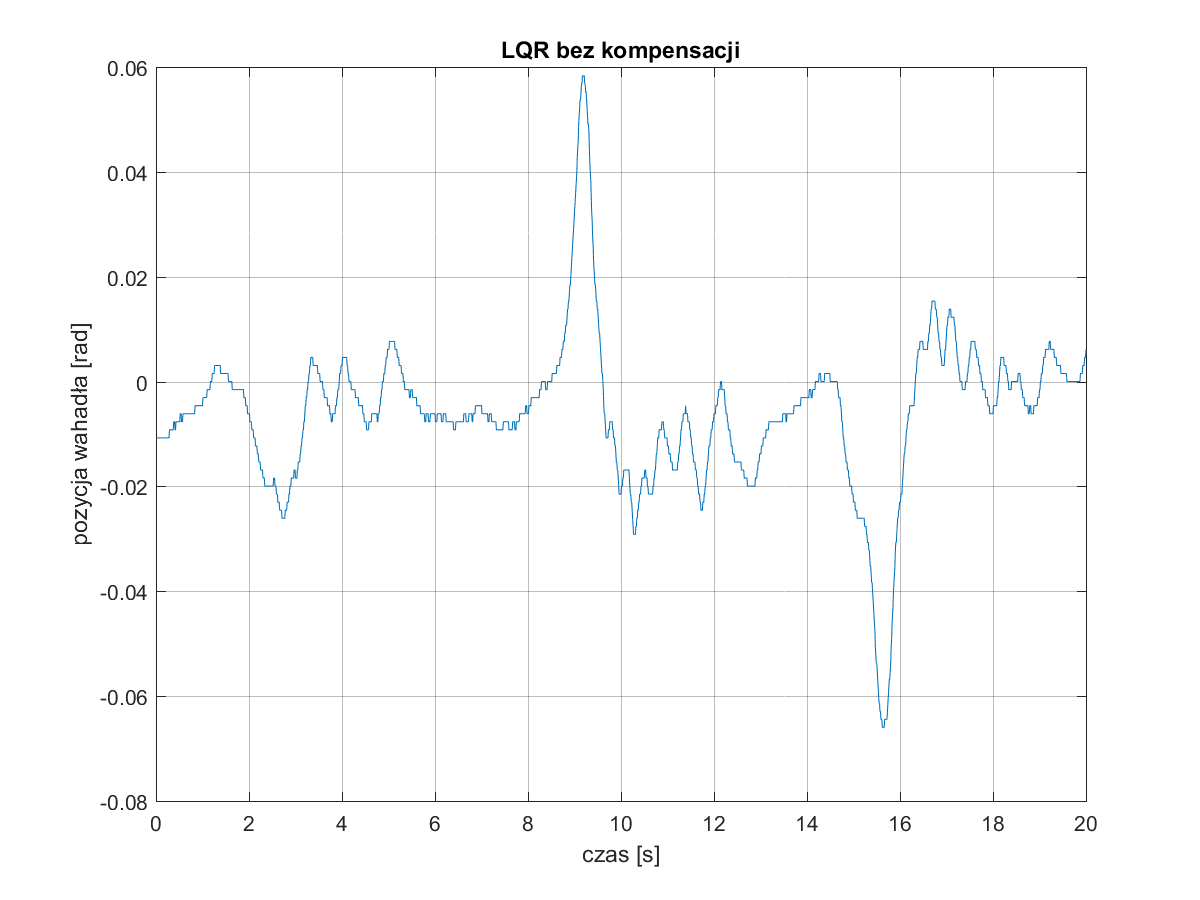
\includegraphics[width=2.8in]{obrazy/pendulum/LQR_bezk_poz_wah.png}}
	\caption{Swing-up wraz ze stabilizacją wahadła, zmiana referencyjnego położenia wózka.}
\label{fig:Swing2}
\end{figure}

\include{Wnioski}
%\input{wyniki}
\newpage
\tableofcontents
\newpage
\nocite{*}
\printbibliography
%\addcontentsline{toc}{chapter}{Bibliografia}
\end{document}